%%   
%% Copyright 2007, 2008, 2009 Elsevier Ltd
%% 
%% This file is part of the 'Elsarticle Bundle'.
%% ---------------------------------------------
%% 
%% It may be distributed under the conditions of the LaTeX Project Public
%% License, either version 1.2 of this license or (at your option) any
%% later version.  The latest version of this license is in
%%    http://www.latex-project.org/lppl.txt
%% and version 1.2 or later is part of all distributions of LaTeX
%% version 1999/12/01 or later.
%% 
%% The list of all files belonging to the 'Elsarticle Bundle' is
%% given in the file `manifest.txt'.
%% 

%% Template article for Elsevier's document class `elsarticle'
%% with numbered style bibliographic references
%% SP 2008/03/01

\documentclass[preprint,12pt]{elsarticle}

%% Use the option review to obtain double line spacing
%% \documentclass[authoryear,preprint,review,12pt]{elsarticle}

%% Use the options 1p,twocolumn; 3p; 3p,twocolumn; 5p; or 5p,twocolumn
%% for a journal layout:
%% \documentclass[final,1p,times]{elsarticle}
%% \documentclass[final,1p,times,twocolumn]{elsarticle}
%% \documentclass[final,3p,times]{elsarticle}
%% \documentclass[final,3p,times,twocolumn]{elsarticle}
%% \documentclass[final,5p,times]{elsarticle}
%% \documentclass[final,5p,times,twocolumn]{elsarticle}

%% For including figures, graphicx.sty has been loaded in
%% elsarticle.cls. If you prefer to use the old commands
%% please give \usepackage{epsfig}

%% The amssymb package provides various useful mathematical symbols
\usepackage{amssymb}
\usepackage{url}
\usepackage{color}
\usepackage{xspace}
\usepackage{graphicx}
\usepackage{wrapfig}
\usepackage{caption}
\usepackage{booktabs}
\usepackage{subcaption}
\usepackage{ifpdf}

%% The amsthm package provides extended theorem environments
%% \usepackage{amsthm}

%% The lineno packages adds line numbers. Start line numbering with
%% \begin{linenumbers}, end it with \end{linenumbers}. Or switch it on
%% for the whole article with \linenumbers.
%% \usepackage{lineno}

\ifpdf
 \DeclareGraphicsExtensions{.pdf, .jpg, .tif, .png}
\else
 \DeclareGraphicsExtensions{.jpg, .png, .ps}
\fi


\newif\ifdraft
\drafttrue
%\draftfalse                                                                              
\ifdraft
\newcommand{\katznote}[1]{ {\textcolor{blue}    { ***Dan:   #1 }}}
\newcommand{\zhaonote}[1]{{\textcolor{cyan}{ ***Zhao:  #1 }}}
\newcommand{\amnote}[1]{{\textcolor{magenta}    { ***Andre: #1 }}}
\newcommand{\jhanote}[1]{{\textcolor{green}    { ***Shantenu: #1 }}}
\newcommand{\note}[1]{ {\textcolor{red}    {\bf #1 }}}
\else
\newcommand{\katznote}[1]{}
\newcommand{\zhaonote}[1]{}
\newcommand{\amnote}[1]{}
\newcommand{\jhanote}[1]{}
\newcommand{\note}[1]{}
\fi

\newcommand{\I}[1]{\textit{#1}\xspace}
\newcommand{\B}[1]{\textbf{#1}\xspace}
\newcommand{\T}[1]{\texttt{#1}\xspace}
\newcommand{\N}{\newline}
\newcommand{\HF}{\hfill}

\journal{FGCS}

\begin{document}

\begin{frontmatter}

%% Title, authors and addresses

%% use the tnoteref command within \title for footnotes;
%% use the tnotetext command for theassociated footnote;
%% use the fnref command within \author or \address for footnotes;
%% use the fntext command for theassociated footnote;
%% use the corref command within \author for corresponding author footnotes;
%% use the cortext command for theassociated footnote;
%% use the ead command for the email address,
%% and the form \ead[url] for the home page:
%% \title{Title\tnoteref{label1}}
%% \tnotetext[label1]{}
%% \author{Name\corref{cor1}\fnref{label2}}
%% \ead{email address}
%% \ead[url]{home page}
%% \fntext[label2]{}
%% \cortext[cor1]{}
%% \address{Address\fnref{label3}}
%% \fntext[label3]{}

\title{Application Skeletons: Construction and Use in eScience}

%% use optional labels to link authors explicitly to addresses:
%% \author[label1,label2]{}
%% \address[label1]{}
%% \address[label2]{}

\author[ucanl]{Daniel S. Katz\corref{cor1}}
\ead{d.katz@ieee.org}

\author[rutgers]{Andre Merzky}
\ead{andre@merzky.net}

\author[ucb]{Zhao Zhang}
\ead{zhaozhang@eecs.berkeley.edu}

\author[rutgers]{Shantenu Jha}
\ead{shantenu.jha@rutgers.edu}

\cortext[cor1]{Corresponding author} 

\address[ucanl]{Computation Institute, University of Chicago \& Argonne National Laboratory, Chicago, IL, USA}
\address[rutgers]{RADICAL Laboratory, Rutgers University, New Brunswick, NJ, USA}
\address[ucb]{AMPLab, University of California, Berkeley, CA, USA}


\begin{abstract}

Computer scientists who work on tools and systems to support
eScience (a variety of parallel and distributed) applications usually use actual applications to prove that their
systems will benefit science and engineering (e.g., improve application performance). Accessing and building the applications and necessary data sets can be difficult because of policy
or technical issues, and it can be difficult to modify the characteristics of the applications to understand corner cases in the system design.
In this paper, we present the Application Skeleton, a simple yet powerful 
tool to build synthetic applications that represent real applications, with runtime and I/O 
close to those of the real applications. This allows computer 
scientists to focus on the system they are building; they can work with the simpler skeleton 
applications and be sure that their work will also be applicable to the real applications. 
In addition, skeleton applications support simple
reproducible system experiments since they are represented by a compact set of parameters.

Our Application Skeleton tool (available as open source at \url{https://github.com/applicationskeleton/Skeleton}) currently can create easy-to-access, easy-to-build, and easy-to-run bag-of-task, 
(iterative) map-reduce, and (iterative) multistage workflow applications. The tasks can be
serial, parallel, or a mix of both. The parameters to represent the tasks can either be
discovered through a manual profiling of the applications or through an automated method.
We select three representative applications (Montage, 
BLAST, CyberShake Postprocessing), then describe and generate skeleton applications for each. 
We show that the skeleton applications have identical (or close) performance to that of the real applications. 
We then show examples of using skeleton applications to verify system optimizations such as
data caching, I/O tuning, and task scheduling, as well as the system resilience mechanism, in some cases modifying the skeleton applications to emphasize some characteristic, and thus show that using skeleton applications 
simplifies the process of designing, implementing, and testing these optimizations.

\end{abstract}

\begin{keyword}
computational science \sep data science \sep application modeling \sep system modeling \sep performance modeling \sep parallel and distributed systems

%% keywords here, in the form: keyword \sep keyword

%% PACS codes here, in the form: \PACS code \sep code

%% MSC codes here, in the form: \MSC code \sep code
%% or \MSC[2008] code \sep code (2000 is the default)

\end{keyword}

\end{frontmatter}

%% \linenumbers

%% main text


\section{Introduction} \label{lb:intro}

Computer scientists who build tools and systems (programming languages, runtime systems, file systems, workflow systems, etc.) 
%to support distributed applications often have to work on real scientific applications to prove the effectiveness of
%\zhaonote{put in the word ``eScience''}
to enable eScience often have to work on real scientific applications to prove the effectiveness of 
the system. Accessing and building the real applications can be time consuming or sometimes infeasible for one
or more of the following reasons:
\begin{itemize}
\item {} Some applications (source) are privately accessible.
\item {} Some data are difficult to access.
\item {} Some applications use legacy code and are dependent on out-of-date libraries.
\item {} Some applications are hard to understand because they implicitly assume domain knowledge.
\end{itemize}

In addition, real applications may be difficult to scale or modify in order to
demonstrate system trends and characteristics. Our work is partially motivated
by the state of distributed applications.  We previously
highlighted the challenges of developing distributed applications, showing that the lack of
development abstractions and the complexity of deployment were two important
barriers~\cite{DPA-paper,dpagrid2009}.
% \jhanote{Maybe we should add a sentence or two
%  -- possibly around the reference to the DPA Paper that we're really interested
%  in distributed applications. This ``detail'' was lost on at least one
%  reviewer. If we do so, we should also add deployment challenges are another
%  motivation for Skeletons} \katznote{please give it a go}\jhanote{OK?}

Our Application Skeletons idea was created in the AIMES project, whose goal is
to explore the role of abstractions and integrated middleware to support
eScience at extreme scales. AIMES is co-designing middleware from an application
and infrastructure perspective. Thus, it requires applications with various
characteristics for better application coverage. We have previously encountered
many problems when accessing real applications and when trying to distribute
applications and data as test cases to other researchers. Application Skeletons
are intended to overcome these issues.

We previously presented~\cite{Skeleton2013} the Skeleton idea of working around such issues by quickly
and easily producing a synthetic distributed application that is executable in a distributed environment, for example, grids, clusters, and clouds, and then showed~\cite{Skeleton2014} improvements in reducing the gap between skeleton and real application performance, as well
as showing Skeleton applications could be used to simplify understanding and demonstrating system optimizations, such as AMFORA~\cite{AMFS2013}.

The Application Skeleton tool takes as input an application description file composed in a top-down approach: an application was described
as a number of stages, and each stage had a number of tasks. Users specify tasks at the stage level by articulating
the number of tasks, task lengths, and input/output file sizes. Applications can be composed of serial tasks, parallel tasks, or a mix of both. The task is implemented as a versatile C program, and the compiled executable can be serial or parallel dependent on how it is compiled. 
Users can specify a task's read/write buffer size, since such buffers are often used in real application code. 
The Skeleton task can mimic real application tasks' interleaving behavior for reads, writes, and computation. 
The tasks are C programs compiled to static executables, so they can run on supercomputers with an OS that doesn't have fork()/exec() support, such as the IBM Blue Gene/Q. 
Some of the task parameters, such as task lengths and input file sizes, can be
described as a statistical distribution.
The task implementation is based on the UNIX/Linux sleep and dd programs, controlling the CPU time and I/O, respectively.

This Skeleton implementation can generate bag-of-task, (iterative) map-reduce, and (iterative) multistage workflow applications. 
The skeleton applications are executable with common
distributed computing middleware, Swift~\cite{SWIFT2007, swift-ieee09, Swift_2011} and Pegasus~\cite{pegasus, pegasus-04}, as well as the ubiquitous UNIX shell on a single 
site (a local cluster with a shared file system), and the skeleton set of tasks can also be output as a generic JSON object that can be used by other systems, such as in our case, by our AIMES middleware.

Skeleton parameters can be discovered by either by manually or automatically profiling the application.
Once the real application is represented by a Skeleton description file, it can easily be distributed and reused.  
We measured the performance error between the skeleton application against three real applications (Montage~\cite{montage1,montage2}, BLAST~\cite{ParallelBlast}, and CyberShake PostProcessing~\cite{SCEC07}) on 64 processors of a BG/P supercomputer with per stage and total errors of between 1 and 3\%.
And changing the parameters makes it easy to study how the system responds to different application characteristics, specifically data caching, task scheduling, I/O tuning, and resilience mechanism.

%Providing an easy-to-use way to specify a Skeleton application with acceptable
%performance difference between Skeleton applications and real applications was the major challenge of this work. In many cases,
%we had to relax the behavioral similarities between it and a real application to promote ease of programming.
%For example, while we want a skeleton task to mimic the exact behavior (operation sequence of computation and I/O) of a real 
%application task, doing so would result
%in reimplementing the actual task and thus eliminating the ease of programming. We therefore provide only a limited number of operation 
%interleaving options that users can choose from. 
%A second challenge is the tradeoff between the ease of programming and expressiveness: we want  Skeletons to cover iterative
%applications, but we don't want to fully implement a new control flow language. As a compromise, an iterative Skeleton application can have only a fixed number of
%iterations over stages; that is, we don't support dynamic convergence checking. 


This paper summarizes our previous work~\cite{Skeleton2013,Skeleton2014} and adds further work towards automated, system independent application profiling. 
Specifically, almost all of Section~\ref{lb:Params} is new, and Section~\ref{lb:RFwork} (related work) has been expanded to provide better context for our work; as such, it also has been moved to earlier in the paper.
Sections~\ref{lb:Design} and \ref{lb:Perf} were initially shortened to focus on key points and then modified to include automated profiling, then further modified as part of the review process.  
The introduction (Section~\ref{lb:intro}) and conclusions (Section~\ref{lb:Con}) have been reworked for this paper but used the introductions and conclusions of the previous papers as starting points.
Section~\ref{lb:using} has just been condensed from~\cite{Skeleton2014}.

The contributions of this work include the following:
\begin{itemize}
\item An application abstraction that gives users good expressiveness and ease of programming to capture the key performance elements of distributed applications
\item A versatile Skeleton task implementation that is configurable (serial or parallel, number of processes, read/write buffer size, input/output files, interleaving options)
\item A comparison of two methods for the estimation
    of Skeleton parameters: manual, system specific application profiling
    versus automated, system independent profiling 
\item An interoperable Skeleton implementation that works with mainstream workflow frameworks and systems (Swift, Pegasus, and Shell), and allow general output for other systems
\item The usage of Skeleton applications to simplify system optimization implementation and highlight their impacts
\end{itemize}

The rest of the paper is organized as follows: 
%Section~\ref{lb:Survey} surveys a number of distributed applications that Application Skeletons are intended to cover. 
Section~\ref{lb:RFwork} discusses the idea of application modeling, including related work.
Section~\ref{lb:Design} introduces the design of the Application Skeleton tool and the tradeoffs we made during the process.
%Section~\ref{lb:Model} presents the Application Skeleton programming model with several examples.
In Section \ref{lb:Params}, we discuss how Skeleton parameters can be determined.
In Section \ref{lb:Perf}, we select three representative applications, and compare the Skeleton application performance against the real application performance. In Section \ref{lb:using}, we show how application skeletons can help eScience infrastructure developers.
Conclusions are drawn in Section~\ref{lb:Con}. 

%\section{A Survey of Distributed Applications}
%\label{lb:Survey}

\section{Modeling Background and Related Work}\label{lb:RFwork}

Researchers have been using application replacements of various types (e.g.,
kernels, benchmarks, reduced applications, mini-apps, traces) for experiments for a long
time, and some of those replacements have been and are certainly tunable in one
way or another. These application replacements are used for a variety of
purposes, including: %\katznote{others?}
\begin{itemize}
\item They are easier to build than the actual application.
\item They can be reused across different system to compare those systems.
\item They run faster than the actual application.
\item They can be shared with collaborators who do not have access to the application or the data. 
\end{itemize}

However, we believe that the idea of using application skeletons, particularly
for overall system performance, is relatively novel.  The distinction in our
work is that the Skeletons provide a systematic application replacement 
capability, which both preserves
the significant part of the application's behavior
and is tunable across a range of diverse
applications. Because of the problem space
is pervasive but attempts to solve it systematically are rare, particularly for
distributed applications, the related work we discuss here are examples of some
of the different types of application replacements that have been used. 

Examples of benchmarking/analysis work in a parallel (not distributed) context
include the NAS Parallel Benchmarks~\cite{NPB}, and Berkeley
Dwarfs~\cite{dwarfs} (also called `motifs') and the related
OpenDwarfs~\cite{6868650}.  The NAS benchmarks include both kernels and
pseudo-applications (an example of reduced applications), intended for use on
parallel (not distributed) computers.  These benchmarks can be scaled by
choosing different predeveloped classes.  However, they cannot be arbitrarily
tuned to expose particular system features, as skeletons can.  The dwarf work
has at its core the idea that there is a key computational or data movement
kernel that is responsible for most of the application's performance, and that
that kernel can be extracted and used to represent the full application, at
least in terms of performance.

Additional examples are from Kerbyson et
al.~\cite{Kerbyson_SC13}, who used simplified version of parallel MPI applications
to study Blue Gene systems; and Worley et al.~\cite{Worley1994,FosterWorley1997}, 
who studied a parallel spectral transform shallow water model by implementing the
real spectral transform in what is otherwise a synthetic code that replicates a
range of different communication structures as found in different parallelizations
of climate models.  Similarly, Prophesy~\cite{Taylor_HPDC2000} is an infrastructure that helps in performance modeling of applications on parallel and distributed systems through a relational database that allows for the recording of performance data, system features and application details.  The applications data gathered has some overlap with the processes by which we can obtain our skeleton parameters.

An alternative to reducing the application over the space of the application is
reducing it over time.  For example, Sodhi et
al.~\cite{Sodhi:2008:PPS:1355774.1355777} developed a tool called performance
skeletons.  These are short running parallel MPI programs with performance meant
to fractionally represent the performance of the full applications.  Unlike the
dwarf work, this assumes that the work done by applications is spread through
out the application (not in a single kernel).  This idea of fractional versions
of parallel applications is also unlike our work, which produces simplified and
scalable versions of full distributed applications.  Our work overlaps with
Sodhi's in its approach to automatically
capturing the execution behavior of an application and automatically generating
a synthetic skeleton program that reflects that execution behavior; however,
Sodhi focuses on single system MPI
applications that do not have disk I/O.

Skel~\cite{Skel} uses a similar idea, though it aims at understanding the I/O performance of parallel applications on supercomputers. Users can extract 
the I/O behavior from an application, then produce a skeletal application that mimics the I/O operations and pattern by specifying
a Skel configuration file. The produced skeletal application can run on ADIOS~\cite{ADIOS}. 

The work that is probably closest to ours is WGL~\cite{WGL}, which abstracts an application from a dataflow point of view and lets users generate a Swift script for a potentially distributed workflow application by 
describing the dataflow patterns between stages.  Since there is some institutional overlap between
the WGL developers and Skeleton developers and because both overlap the Swift team, it's likely that informal discussions carried some of this concept from WGL to Skeletons, though there is a nine-year gap between the projects.

Another application replacement is system traces, used when the analyzers do not have access to the applications or the data.  Some examples of system traces can be found in:
Chen et al.~\cite{MRTraces2012}, who analyzed a collection of industrial MapReduce workload traces and built a big data processing benchmark for MapReduce systems;
Harter et al.~\cite{HDFSTraces2014}, who studied the underlying HDFS traces to understand the performance of the Facebook message service, then proposed potential improvements; and
Ousterhout et al.~\cite{SparkTrace2015}, who analyzed the Spark traces of industrial applications to study potential improvements of potential hardware upgrades.

Loosely related work includes Holl et al.~\cite{Holl:2013:SSS:2534248.2534251}, who have studied how to store and share parameters values for shared workflows, an idea that could be applied to skeleton values; and algorithmic motifs (formerly called skeletons)~\cite{foster1990parallel}, which abstracts parallel application with an algorithmic approach, and lets users build parallel programs based on the algorithmic motifs.  The term skeleton has also been used in SKOPE, which produces a descriptive model about the semantic behavior of a workload, which can infer potential transformations and help users understand how workloads may interact with and adapt to emerging hardware. SKOPE models can be shared, annotated, and studied by a community of performance engineers and system designers.



\section{Application Skeleton Design}

%\katznote{how much of this can we remove and just point to the previous workshop paper?} 
\label{lb:Design}
In addition to the design of application abstraction, stage characterization, and task configuration, the Application Skeleton's design involves
other aspects, such as system tool compatibility and platform interoperability, to make it easy to build, easy to run, and easy to change. This section discusses
the requirements in detail, the problems we encountered during the design process, and how we met those requirements and overcame the
problems.

We are motivated by a wide variety of eScience application types for which we want to be able to build representative skeleton applications. The Application Skeleton implementation
currently allows the user to express the following:
\begin{itemize}
\item {Bag of Tasks}: A set of independent tasks. Examples: MG-RAST~\cite{MG-RAST}, DOCK~\cite{dock5-06}
\item {MapReduce}: A set of distributed application with key-value pairs as intermediate data. Examples: high energy physics histograms~\cite{SCIMP}, object ordering~\cite{PageRank2}
\item {Multistage Workflow}: A set of distributed applications with multiple stages using files for intermediate data. Examples: Montage~\cite{montage1}, BLAST~\cite{ParallelBlast}, CyberShake postprocessing~\cite{SCEC07}
\item {Iterative MapReduce}: MapReduce with iterations. Example: %linear algebra~\cite{MadLINQ},
graph mining~\cite{PREGEL}
\item {Campaign}: An iterative application with a varying set of tasks that must be run to completion in each iteration. Example: Kalman filtering~\cite{KALMAN}
%\zhaonote{can we cover Campaign now? If my understanding is correct, we can now.}
\end{itemize}

Application Skeletons of iterative applications are currently limited to those with a fixed number of iterations. Also, Application Skeletons  can express multiple task types, serial, parallel, or a mix of both. 
Examining several representative distributed applications, we observe
that abstracting a distributed application stage by stage is expressive enough to cover the target applications.
The Application Skeleton concept ideally should also allow a concurrent application (a set of tasks that have to be executed at the same time, e.g., coupled fusion simulation~\cite{klasky:journphy:2005}) to be expressed; this is future work.

%\subsection{Application Abstraction}
%\label{lb:Design:App}
%\zhaonote{data flow, control flow, application type (serial, parallel, mixed)}
%Application Skeletons can represent a group of distributed application types: bag-of-task, (iterative) map-reduce,
%and (iterative) multi-stage workflow, where iterative applications are currently limited to those with a fixed number of iterations. Application Skeletons also can express multiple task types. The skeleton application 
%can be composed of serial tasks or parallel tasks or a mix of both.


%\zhaonote{maybe we can remove the paragraph below. It is arguing that abstracting application from stage is expressive enough.}
%Bag-of-tasks, which is composed of a number of independent tasks without data or control dependencies, is naturally a single stage of computation.
%Map-reduce can be divided into a map stage and a reduce stage. (There is also a shuffle stage involved implicitly in many system implementations.)
%Workflow applications, which are often represented as a DAG, often can also be abstracted as a set of computation stages.
%The iterative versions of map-reduce and workflow applications run computation stages multiple times. 

%\zhaonote{the following paragraph can be replaced by saying "Application Skeletons support iterative applications with a fixed number of iterations."}
%In some cases, iterative applications run for a fixed number of iterations, while in others, the iterations continue until some
%condition is reached. Ideally, we would like Application Skeletons to cover both cases. However, implementing the iteration termination
%based on condition checking requires the implementation of the whole control flow logic, which would lead Application Skeletons to become a complete
%programming language. So we decide to only support the iterative applications with a fixed number of iterations.

%\zhaonote{the following paragraph can be replaced by saying "Application Skeletons now can support both serial and parallel task."}
%We aim to represent applications that are composed of multiple task types: serial, parallel or a mix of both. 
%Some applications may contain some serial tasks while the others are parallel in one stage. 
%From a conceptual data flow point of view, those
%tasks belong to one stage. However, designing Application Skeletons in exactly this way would result in poor programmability. So in our design,
%an Application Skeleton stage has a single task type, either serial
%or parallel. To represent applications with both types of tasks in a stage, one can describe two computation stages, with serial and parallel task respectively. Since the
%data dependencies remain the same, these two stages are still one virtual stage if we look at the data flow graph. And a system tool that resolves
%task dependencies at the file level (e.g. Swift) will be able to launch both stages simultaneously.

\subsection{Task Configuration}
The core elements of tasks are computation and I/O. In the Application Skeleton
design, time consumption of computation is represented by letting the task sleep
for a user-specified period.  A serial task only mimics the computation and I/O,
since in many applications the communication between tasks is in the form of
file production and consumption. Tasks with communication between processes
(within a task) are referred to as parallel tasks.
%Parallel tasks can mimic the computation and I/O operations, 
%while the communication within tasks are simplified as a barrier before the task exits. 
%\katznote{last part is a little hard to understand}
%A Skeleton parallel task simplifies the computation and I/O by let only one process mimic the operations, while other processes simply sleep. Right before the parallel task exits,
%there is a barrier called to make sure all operations on all processes have finished.
%\zhaonote{rephrased, please review}
%\katznote{we say this later; I don't think we need it here too}

An Application Skeleton task is implemented as a standalone C program. It  requires only the standard math library and MPI library to preserve the
portability. A serial task can be compiled with a standard C compiler, while a parallel task needs to be compiled with an MPI C compiler. Users specify the task type in the stage description, and the Application Skeleton tool will produce 
a compilation script that can compile the task code.

Other task properties include number of processes, task length, read buffer size, write buffer size, input files, output files, and
operation interleaving option. The number of processes is one if the task is serial and is greater than one if the task is parallel. 
Task length is currently measured in seconds, which reflects the amount of computation in a task. 
Section~\ref{ssec:si_profiling} discusses the tradeoffs between this approach and an
alternative representation of compute load, via FLOPs.

A serial task reads input files, sleeps (to represent computation), and writes output files. In a parallel task, the rank 0 process reads
input files, sleeps (in place of computation), then writes output files, while other processes simply sleep for the computation time length.  All processes (including rank 0) wait at a barrier before the task exits. 
%\katznote{is 'does computation' different than 'sleeps'?} 
%\zhaonote{No, 'does computation' is exactly spleeping. I add one more sentence in the first paragraph of this subsection to explain computation is in the form of sleep}
%There is a barrier point in every process before the program exits.

We want to balance between mimicking the exact the operation sequence of the real application tasks' I/O and computation in the skeleton task and having very simple programming.  The former requires reimplementing the actual task and results in poor programmability, while the latter gives very different performance.  As a compromise,
 we define four interleaving options for a skeleton task (the serial task or the rank 0 process in a parallel task): %, as visualized in Figure~\ref{fig:interleave}:
\begin{enumerate}
\item[0.] \textbf{interleave-nothing}: reads, computes, then writes
\item{\textbf{interleave-read-compute}:} interleaves reads and computations, then writes outputs
\item{\textbf{interleave-compute-write}:} reads all inputs, then interleaves writes and computations
\item{\textbf{interleave-all}:} interleave reads, computations, and writes
\end{enumerate}

%\begin{figure}[h]
%\begin{center}
%    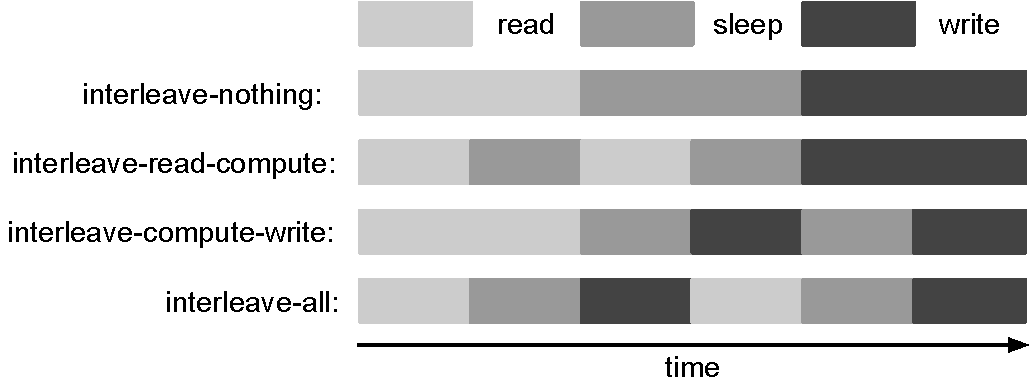
\includegraphics[width=85mm]{pictures/Interleave}
%\caption {Visualization of the Interleaving Options
%    \label{fig:interleave}
%}
%\end{center}
%\end{figure}

%Users do not have to specify the task configurations for each individual task. Instead, the automatic configuration is done at the stage level, 
%where there is a better global view of many properties. 
%\katznote{is this a paragraph by itself, or is it part of the previous one?  and is it different from the next paragraph?}
%\zhaonote{I was thinking that after reading so much about task configuration, a reader might think he is going to specify every single task in Skeleton, so I put
%this paragraph here to avoid that. I think we can also remove it, since we talk about it in the next subsection.}

\subsection{Stage Characterization}
\label{ssec:stage_char}
We have previously shown basic examples of applications described using the Skeleton programming model~\cite{Skeleton2013}.
In brief, we specify the task parameters at the stage level since it has a fairly global view of most of the task
properties, which eases programming over specifying each task's parameters individually. The stage parameters are:
\begin{itemize}
\item{\textbf{Stage\_Name}:} the stage name %The tasks of this stage are named: \$\{Stage\_Name\}\_\$\{Task\_id\}. (This is particularly useful when when external mappers are used)
\item{\textbf{Stage\_Type}:}  the type of the tasks, serial or parallel
\item{\textbf{Num\_Tasks}:}  the number of tasks
\item{\textbf{Num\_Processes}:} the number of processes per task
\item{\textbf{Task\_Length}:}  the length of the tasks
\item{\textbf{Read\_Buffer}:} the read buffer size in the task
\item{\textbf{Write\_Buffer}:} the write buffer size in the task
\item{\textbf{Input\_Files\_Each\_Task}:}  the ratio between number of input files and the number of tasks
\item{\textbf{Input\_Source}:}  the source of the input files, either filesystem or outputs of a previously defined stage
\item{\textbf{Input\_File\_Size}:}  input file size for the stage, with distribution: uniform, normal, triangular, or lognorm
\item{\textbf{Input\_Task\_Mapping}:} user-specified input file and task mapping, to support external mapping, letting the user override the mapping scheme implied by \textbf{Input\_Files\_Each\_Task}
\item{\textbf{Output\_Files\_Each\_Task}:}  the number of output files per task in the stage (multiple tasks writing to one file are not currently supported)
\item{\textbf{Output\_File\_Size}:}  the output file size
\item{\textbf{Interleave\_Option}:} the interleaving option of the task
\item{\textbf{Iteration\_Num}:} optional parameter specifying the number of iterations
\item{\textbf{Iteration\_Stages}:} the names of the other stages involved in the iteration
\item{\textbf{Iteration\_Substitute}:} the input file in tasks that will be replaced in the second and later iteration % (e.g., ``Stage\_1.output 1'' replaces the first input file of the tasks in Stage\_1 with its output files). 
\end{itemize}

Task\_Length, Input\_File\_Size, and Output\_File\_Size can be stated as statistical distributions. The Application Skeleton tool currently supports uniform, normal, triangular, and lognorm distributions. Task\_Length 
can also be specified as a polynomial function of Input\_File\_Size (of the first input file). Similarly, Output\_File\_Size
can be specified as a polynomial function of Input\_File\_Size (of the first input file) or Task\_Length.


\subsection{Mapping Files and Tasks}

%Line 27 and 40 in Listing~\ref{lst:sample} specify the input file mapping option for the second and
%third stage respectively.
Instead of declaring every input file's source and size, we describe
the mapping with a combinatorial function,
{\it combination Stage\_1.Output 2},
 interpreted as follows: choose two of the output files of Stage\_1 as input files for each task.
Choosing two from $N$ files can have $N \choose 2$ different file combinations. 
%\katznote{so which is chosen?}
%\zhaonote{add some explanation}
For example, choosing two files from \{output\_0, output\_1, output\_2, output\_3\} returns six pairs of files: 
\{output\_0, output\_1\}, \{output\_0, output\_2\}, \{output\_0, output\_3\}, \{output\_1, output\_2\}, \{output\_1, output\_3\}, and \{output\_2, output\_3\}.
These six file pairs will be assigned to six tasks, so if there are six tasks, each will get a distinct file pair as its input files. (If there are more than six tasks, inputs will be repeated.)
%\katznote{so the number of tasks that consume the files needs to match the size of $N \choose 2$ for this to be unique?}
%\zhaonote{the mapping is unique if the number of tasks is equal or less than $N \choose 2$, otherwise, we  will see tasks with the same set of input files.} \katznote{huh?  what does `we  will see tasks with the set of input files' mean?}\zhaonote{oops, I mean the same set of input files.}

Another Input\_Task\_Mapping option is {\it external}. Here, a user-specified
shell script or a Python function will be called by the Application Skeleton tool. An external script
has to print the input files names of a task in a line, and a Python function needs to return a nested
list of input file names.

If the user specifies the source of the input files of the second stage as the output of the first stage
but does not use the Input\_Task\_Mapping option, then the files are mapped to each task sequentially: the first and second file are mapped to the first task, the third and fourth file are mapped
to the second task, and so on. If the mapping runs out of input files, it will go back to the beginning
of the input file list, and multiple tasks will consume some input files.

%\subsection{Task Specification}
%\zhaonote{this subsectino can be removed too, we have explained the idea in previous section. This is tech details.}
%At the task level, the Application Skeleton tool parses the input application description file and writes the
%task command lines in a Bash script for each stage, for example:
%\begin{shortlist}
%\item[] /path/to/task task\_type num\_processes task\_length \\
%read-\_buffer write\_buffer num\_input num\_output \\
%interleave\_opt input\_filename [input\_filename...] \\
%output\_filename output\_file\_size [output\_filename \\
%output\_file\_size...] 
%\end{shortlist}
%All the task parameters are determined by the stage parameter specification.
%If task length and file size settings are needed that are beyond the Application Skeleton tool's capability, customized scripts that generate the tasks with the above format can be used.

\subsection{Iteration Support}
%\zhaonote{newly added, please review}
%\katznote{this is all details we either don't need or have already said}
%The application generation command is in the following format:
%\begin{shortlist}
%\item[] skeleton.py app\_desc.input output\_format output\_prefix site\_desc.input
%\end{shortlist}
%Assumming the description file's name of the three stage workflow example in Listing~\ref{lst:sample} is multi-stage.input.
%The actual command to generate the application is:
%\begin{shortlist}
%\item[] skeleton.py multi-stage.input Shell multi-stage local.input
%\end{shortlist}
%The site description file requires users to specify a couple of parameters of each site that the synthetic application
%will run on. The format of site description file is csv, users specify the site name, compiler path, compiler flags, 
%and remote the directory where the task will be compiled remotely. Listing~\ref{lst:site} shows an example to describe
%the local site. We use two lines for each site, with one line specifying the options to compile serial task and the other
%line referring to parallel task.
%
%\begin{lstlisting}[caption=An Example of Local Site Description, label=lst:site, linewidth=1.0\textwidth, xleftmargin=2.5ex]
%localhost, gcc, -lm, /home/skeleton/
%localhost, mpicc, -DMPI -lm, /home/skeleton/
%\end{lstlisting}


%With the description file in Listing~\ref{lst:sample}, the Skeletons generate three
%preparation scripts (in Bash, one for each stage), two compilation scripts (one for serial task and the other for parallel task),
%and three application scripts (one for each stage). Now, users can execute the preparations scripts to produce the input/output
%directories and the initial input files. Then users call the compilation scripts to compile the tasks. If there are remote sites
%involved, users need to transfer the task source file and compilation scripts to each remote site, and call the compilation scripts
%on each site. The last step is to launch the application scripts. 

%\zhaonote{proposed text below, please review}
While many multistage workflows execute 
each stage once, some involve iteration, which we had not previously implemented~\cite{Skeleton2013}. Application Skeletons now supports one or more stages that are executed a fixed number of times. 
%\katznote{now we need to say what we have done to make this happen.  How do users specify it.  What do we do then. } % Does the next small paragraph help?  Or is it old and should be removed?}
%Application Skeletons let users specify an iteration of multiple stages for a fixed number of iterations. 
The optional Iteration\_Num parameter declares the number of times a single stage should be executed.
If Iteration\_Num is used, Iteration\_Stages optionally specifies which stages are included in this iteration in addition to the current stage, and
Iteration\_Substitute optionally specifies which input file of the tasks in the current stage will be replaced in the second and later iterations.
%
Iteration support in Application Skeletons requires that the number of output files of the last
stage in the iteration be the same as the the number of initial input files that are going to be replaced in the iterations.
%Application Skeletons does strict checking on the file numbers and exits exceptionally if these two numbers are not equal.

One example is a single stage that iterates three times with the 
first input file for all tasks in this stage replaced by the output files from the previous iteration, after the first iteration. Application Skeletons uses the iteration 
number to differentiate the output files from each stage. In the first iteration, the stage consumes the input files
declared in description (e.g., Stage\_1\_Input) and produces output files with names that include the iteration 
number (e.g., Stage\_1\_Output\_Iter\_1). Starting with the second iteration, the stage consumes the output files from the previous
iteration and increases the iteration number, then produces the outputs. In the last iteration,
the synthetic stage produces output files with the names that are declared in the application description file.

%Iterating over multiple stages depends on Iteration\_Stages, which specifies which stages to iterate. Iteration\_Substitute is again used to replace the input files in the second and later iterations  with outputs of the previous stage.



%\katznote{what happens for input and output files in this case?  Imagine we run Montage with mAdd repeated twice.  What inputs are used the second time?  What is the second output?}
%\zhaonote{A good catch! I was thinking enough about data. In the solution in the current text, the second iteration will take the input exactly as the first iteration, and their outputs overlap too. I think we could add another iteration option, telling the first stage of the iteration which set of files to take as input: Iteration\_intermediate = Stage\_2.Output }
%\katznote{this seems a bit too simple.  Maybe we need something where an iteration number is added to a file?  maybe the first iteration uses the input file as specified and the last output writes the output file as specified, but others would substitute the file names somehow.  I think we need to write down and work through an example of how this would work (outside of the paper) before we decide what to write in the paper}

%\katznote{overall, is this better than just saying that the user could specify a stage multiple times in the script?}
%\zhaonote{Oh, I thought that generating application stage by stage idea was to let users specify the iterations in the script. But it seems not. Could you explain a bit about this solution? Does it mean the skeleton only generates application in stages, and users then modify the Bash or Swift script to support iterations?}
%\katznote{I just meant that rather than the user saying that Stage 3 iterates 2 times, they could just add a Stage 4 that's a duplicate of Stage 3. I guess the main advantage is that our way is a bit easier to write, if we can figure out the data part.}

%With these two iteration parameters, Application Skeletons can generate an iterative application (in the form of Bash script, Pegasus DAG, and Swift script) 
%with an iteration over one stage and multiple stages.
%User can specify the iterative option when calling Applications Skeleton as shown in the example below:
%\begin{shortlist}
%\item[] skeleton.py app.desc output\_format output\_prefix site.desc {\bf iterative}
%\end{shortlist}
%\katznote{this isn't a manual, we don't need calling sequences...}
%The Application Skeleton tool can be run with an iterative flag set.
%Instead of producing the whole application in a single Bash script, Pegasus DAG or Swift script, 
%Application Skeletons will produce a number of Bash scripts, Pegasus DAGs or Swift scripts, with one script for each stage. 
%Users can then launch the script or DAG corresponding to a specific stage multiple times to mimic the iterative
%behavior of the real application.
%\katznote{I thought we agreed this wasn't a good solution, and we wanted a single DAG / script for the application}
%\zhaonote{yes, how about using this solution: for each stage, we define an iteration option, where user can specify the number of iterations of this stage. 
%The user can also specify with which stage, the current stage iterate with. So this covers iteration over a single stage, and over multiple stages. And we can produce Bash, Pegasus, and Swift script accordingly.} \katznote{yes, that sounds good}
%\zhaonote{proposed new text, please review}



%Similarly in the case with Pegasus and Swift, Application Skeletons generate one Pegasus DAG or Swift script for each
%stage in the description file. To run the synthetic application in an iterative way, an application script can be launched
%for several times.

%\zhaonote{this is a bit different with what we did before. To support iterative applications, this is a easier way to specify in all
%Shell, Pegasus, and Swift. We can also generate one DAG or Swift script for the whole application, but I have no idea how to insert
%iterations. So I took one step back, and generate one DAG or Swift script for each stage. This solution places an implicit barrier 
%between stages, which makes it infeasible for Swift/Pegasus developers to work in a barrier-less way. } 
%\katznote{I don't really like this.  I think we need to create a single DAG or Swift script.  And I think this section should go back to just talking about iteration support...}
%\zhaonote{I have the same feeling. So let's do the whole application in the old way, and this way is the special case for iterative applications.}
%\zhaonote{Shall we talk somewhere about the remote site support? (the commented out text)} \katznote{we already do at a high level in \S3.4}

\subsection{System Tool Compatibility and Multiple Sites}
The Application Skeleton tool is implemented with Python, compatible with both Python2 and Python3.  
It reads an application configuration file, parses the text, and sets parameters for each stage.
It then generates three types of files on the local site where it is launched:

\begin{itemize}
\item[] \textbf{Preparation scripts}, to produce the input/output directories and input files for the Skeleton application
\item[] \textbf{Compilation scripts}, to compile the task source code into executables 
\item[] \textbf{Application}, the overall skeleton application, which can be implemented in one of three formats: a plain Bash shell script, with the command lines of each stage in a distinct script file; or a Pegasus DAG task description, with task, data and dependency declaration generated automatically; a functional Swift script that represents the complete application. 
\end{itemize}



This design works well on a single site, such as a single computer or a local homogeneous architecture cluster with a shared file system. However, we also need to support distributed environments, such as running one application on multiple sites, where the sites can have
heterogeneous architectures, resulting in difficult task compilation and deployment. We address this  issue by asking the user for site-specific
information; site-specific information includes site name, serial C compiler path, MPI C compiler path, compilation 
flags, and working directory. Then the Application Skeleton tool generates compilation scripts for each site. Those scripts are run on the remote machines to transfer
the task source code and compile it. 
%And users need to preserve the working directories consistency in the Application Skeleton and system tools such as Pegasus and Swift.

%\section{Skeleton Programming Model}
%\label{lb:Model}
%

%\katznote{again, how much of this can we remove and point to the workshop paper}
%\zhaonote{I think we can remove the subsection below, as it is mostly the same as the example we showed in the workshop paper.}
%%\zhaonote{introduce the programming interface}
%In this section, we introduce the programming model of the Application Skeleton stage and task, and explain file mapping.
%
%\subsection{Stage Specification}
%Specifying a Skeleton application starts with declaring the number of stages, as shown in the configuration file fragment in Listing~\ref{lst:stages}. 
%
%\begin{lstlisting}[caption=Declaring Number of Stages, label=lst:stages, linewidth=1.0\textwidth, xleftmargin=2.5ex]
%Num_Stage = 3
%
%Stage_Name = Stage_1
%    ...
%Stage_Name = Stage_2
%    ...
%Stage_Name = Stage_3
%    ...
%\end{lstlisting}

%\begin{table*}[ht]
%\begin{center}
%\caption{Skeleton Parameter Format}
%\label{tb:parameter}
%\vspace{4pt}
%    \begin{scriptsize}
%\begin{tabular}{|c|c|p{2.5cm}|p{7.5cm}|}
%\hline
%Parameter & Format & Example & notes  \\
%\hline
%\hline
%Task\_Type & String & serial & the only options are serial and parallel\\
%\hline
%Num\_Tasks & Integer & 16 & \\
%\hline
%Task\_Length & dist [parameter][unit] & uniform 32s & other dists: normal, triangular, lognorm\\
%\hline
%Num\_Processes & Integer & 1 & 1 for serial tasks, other integers for parallel tasks\\
%\hline
%Read\_Buffer & Integer & 65536 & the buffer size is measured in bytes\\
%\hline
%Write\_Buffer & Integer & 65536 & the buffer size is measured in bytes\\
%\hline
%Input\_Files\_Each\_Task & Integer & 2 & \\
%\hline
%Input\_\${fileid}.source & filesystem|Stage\_\$.Output & Stage\_1.Output & \\
%\hline
%Input\_\${fileid}.size & dist [parameter][unit] & uniform 1048576 & the default unit is byte, other dists available\\
%\hline
%Input\_File\_Size & dist [parameter][unit] & uniform 1048576 & the default unit is byte, other dists available\\
%\hline
%Input\_Task\_Mapping & option parameters & external map.sh | combination 2 & the external mapping script prints the input files of a task in one line; the combination option choose a number of files from the source with a combinatorial function, if this option is specified, it will overwrite the per file source and size declaration\\
%\hline
%Output\_Files\_Each\_Task & Integer & 2 & \\
%\hline
%Output\_\${fileid}\_Size & dist [parameter][unit] & uniform 1048576 & the default unit is byte, other dists available\\
%\hline
%Interleave\_Option & Integer & 0 & 0--interleave nothing, 1--interleave read and computation, 2--interleave computation and write, 3--interleave all \\
%\hline
%\end{tabular}
%\up
%    \end{scriptsize}
%\end{center}
%\end{table*}

%\begin{lstlisting}[caption=Sample input for a three-stage application,
%%\zhaonote{This following code shows my latest thought about task and input mapping. In Stage2, we call the combination mapping option to tell the skeleton use N choose 2 to map the input files, and this option overwrites the individual file source and size declaration. In function N choose M, M has to be smaller or equal to the number of input files per task. Please review} \katznote{is this a unique mapping?},
%label=lst:sample, linewidth=1.0\textwidth, xleftmargin=2.5ex, basicstyle=\ttfamily\scriptsize]
%Num_Stage = 3
%
%Stage_Name = Stage_1
%    Task_Type = serial
%    Num_Tasks = 4  
%    Task_Length = normal [10, 1]s
%    Num_Processes = 1
%    Read_Buffer = 65536
%    Write_Buffer = 65536
%    Tasks_Each_Input_File = 2
%        Input_1.Source = filesystem
%        Input_1.Size = normal [1048576, 1]B
%        Input_2.Source = filesystem
%        Input_2.Size = uniform 1048576B
%    Output_Files_Each_Task = 1
%        Output_1.Size = normal [1048576, 1]B
%    Interleave_Option = 0
%
%Stage_Name = Stage_2
%    Task_Type = serial
%    Num_Tasks = 6
%    Task_Length = uniform 32s
%    Num_Processes = 1
%    Read_Buffer = 65536
%    Write_Buffer = 65536
%    Input_Files_Each_Task = 2
%    Input_Task_Mapping = combination Stage_1.Output 2    
%    Output_Files_Each_Task = 1
%        Output_1.Size = uniform 1048576B
%    Interleave_Option = 0
%
%Stage_Name = Stage_3
%    Task_Type = serial
%    Num_Tasks = 1
%    Task_Length = uniform 32s
%    Num_Processes = 1
%    Read_Buffer = 65536
%    Write_Buffer = 65536
%    Input_Files_Each_Task = 6
%    Input_Task_Mapping = combination Stage_2.Output 6
%    Output_Files_Each_Task = 1
%        Output_1.Size = uniform 1048576B
%    Interleave_Option = 0
%\end{lstlisting}
%
%\begin{figure}[h!]
%   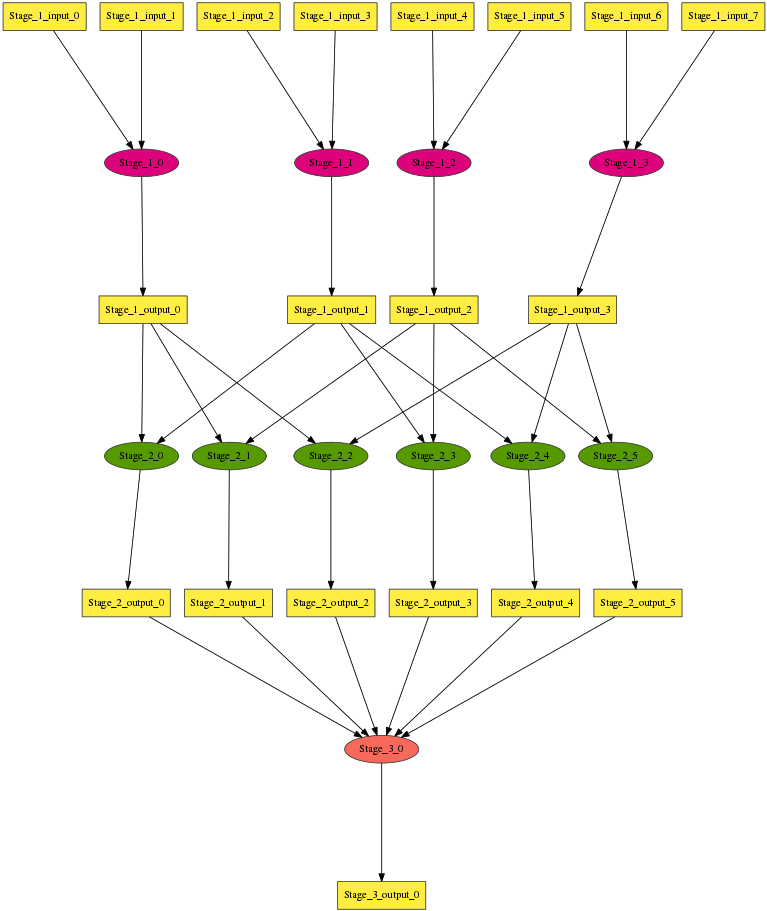
\includegraphics[width=85mm]{pictures/sample}
%\caption {Task flow of the three-stage application
%%\katznote{does this figure match the listing?}
%%\zhaonote{I gave it a double check, I fixed a couple of typos. It most likely matches the listing. We won't be able to confirm this until the whole system is reimplemented. My check is based on our previous Skeleton implementation.}
%   \label{fig:sample}
%}
%\end{figure}
%
%Listing~\ref{lst:sample} shows a complete three-stage application description file, with
%the task flow of the skeleton application presented in Figure~\ref{fig:sample}.
%%Table~\ref{tb:parameter} 
%%\katznote{I don't think we need both table 1 and the list in \S3.3  I suggest we remove the table} 
%%\zhaonote{yes, removed}
%%explains the required data type and format of the parameters. 
%
%The first stage has four serial tasks. The runtime of each
%task conforms to a normal distribution, described by a two-value tuple: [average, stdev]Unit.
%Since they are serial tasks, the number of processes has to be one.
%The read and write buffer are set to 65,536 bytes respectively. 
%Each task reads two input files, and those input files reside on a file system.
%The sizes of all first input files of the tasks conform to a normal distribution, while the sizes of
%all second input files have uniform size of 1048576 bytes.
%Each task writes one output file, with uniform size of 1048576 bytes.
%The Interleave\_option is set to 0, indicating that the task will do the reads, computation, and writes
%in a non-overlapped manner.

\section{Determining Skeleton Parameters}
\label{lb:Params}

In this section, we describe how Skeleton parameters are determined, both manually and
automatically.  We also discuss how automatic generation of Skeleton parameters can lead
to Skeletons that are system independent.

\subsection{Manual Application Profiling}
\label{sec:manual-profiling}

Skeleton parameters can be determined by manually running and analyzing an application.
Specifically, to measure task length, we place both input
and output files on RAM disk and use \T{`time'} to measure the time-to-solution of the tasks.
Although this method includes the I/O
time from/to RAM disk as part of the task length, this extra time is generally negligible
compared with the I/O time using shared disk, which involves
high-volume traffic and high concurrency.
After gathering this data, it can be examined to determine
the average task length and variance, and this can then be used to generate the skeleton
parameters that give the needed task length distribution.
\T{`strace'} is used to profile the I/O traffic, determining the number of reads and writes
and the amount of data
that is read and written by a task.
As we have shown previously~\cite{ENVELOPE}, I/O-related system calls
of all tasks in a stage can be aligned using sequence order. By assuming all tasks get to the
same system call at the same time, I/O concurrency and I/O buffer size can be determined.
This also can be used to determine the interleaving pattern between computation and I/O.  
While this process is manual and a bit time-consuming, it
has also proven to generally be successful~\cite{Skeleton2014}, though with some modifications needed, as described in Section~\ref{lb:Perf}.


\subsection{Automated Application Profiling via SYNAPSE}

The process of manual application profiling as described in
Section~\ref{sec:manual-profiling} is time consuming.  As an alternative
approach, we investigated the use of \I{SYNAPSE}~\cite{review_synapse_wrap,
  synapse-software}, an automated application profiler and emulator.  While
SYNAPSE requires specific system preparations for its profiling step
(specifically Linux kernel support for low level hardware counters), it fully
automates the application profiling at a comparable level of granularity as the
manual approach.  In many ways, it is complementary to the work described
in~\cite{ENVELOPE}: the latter introduces the notion of a \I{system's 
envelope} to describe  system performance in an
application independent way, whereas SYNAPSE describes application performance
independent of the system's envelope, by focusing on system
independent performance metrics. 
%
%\jhanote{Andre: system's envelope is
%  unclear. Please clarify} \amnote{addressed (I hope).}\jhanote{Unfortunately,
%  I'm still not sure what envelope is referring to. System properties?  System
%  specifics?}\amnote{Is it clearer now?}


\subsection{System Independent Profiling}
\label{ssec:si_profiling}

Most, but not all, of the application characteristics listed in
Section~\ref{ssec:stage_char} are system independent, i.e., they have values
that allow faithful reproduction of application behavior on target systems.  For
example, the data input size (in Bytes) is constant, whether the application is
executed on a local desktop, on a remote cluster, or on a supercomputer.  Some
metrics are, however, not system-independent.  Specifically, the application
runtime depends on the specific resource performance, such as the CPU type and
clock speed.

The underlying reason is that some metrics do not really denote metrics of
\I{resource consumption}, but rather describe the \I{effect} of that
consumption.  This is most evident for a metric which is specified as time
duration or frequency, but it can similarly apply to the concurrency of disk
I/O, memory I/O, network I/O and computation, whose realization and performance
can depend on the underlying system architecture.  For example, the manual
application profiling described in Section~\ref{sec:manual-profiling} outlines
how RAM disks are used to separate the effects of I/O on concurrent computation
-- exactly because the computation is measured as runtime, which is influenced
by the overall system performance and load.

SYNAPSE addresses this by estimating the number of FLoating-point OPerations
(FLOPs\footnote{We use \I{`FLOPs'} as the plural of \I{`1 FLOP'},
  vs. \I{`FLOPS'} as \I{`FLoating-point OPerations per Second'}.}) performed by
the application, which represents its compute resource consumption, and which is
thus independent of the specific target system's architecture, configuration,
and load.  While it would be interesting to apply similar system independent
metrics to other resources types (for example, as mentioned, the I/O-Compute
concurrency), we found it difficult to extrapolate the respective parameters
without a complete model of the hardware and OS layer. Without resorting to code
inspection, it is difficult to distinguish if I/O concurrency on the physical
layer is caused by explicit instructions from the application, or by caching and
latency hiding in the operating system layers.

% We also found those effects to be small compared to the other
% characteristics used: the system dependent metrics for those seem to
% be fairly portable, at least for the applications and resources used in our
% experiments. CPU consumption is the only metric we've found worth
% formulating system-independently.  \amnote{this argument needs to be
% improved, and verified with some numbers.  It mostly boils down that
% concurrency between I/O and compute maps nicely to the hardware level
% concurrency which modern systems have, apart from edge cases like I/O
% or network dominated applications.}

\begin{wrapfigure}{l}{0.5\textwidth} \centering
  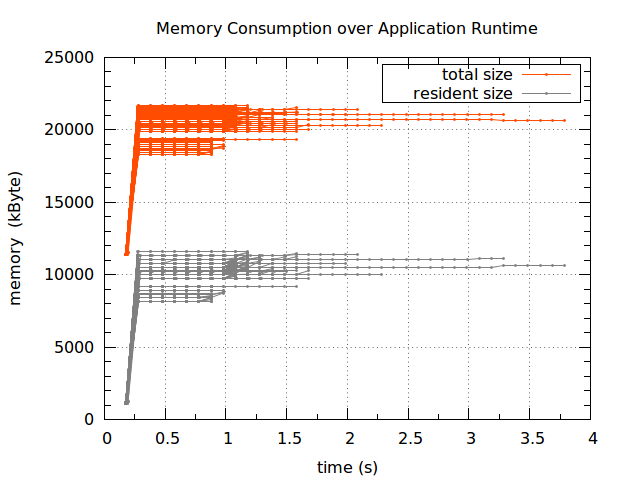
\includegraphics[width=0.5\textwidth]{experiments/synapse_montage/rs_synapse_2mass_m101_j_6_6_mprojectpp_mem}
  \caption { \footnotesize \B{Memory consumption profiles for Montage
      \T{mProjectPP} tasks:} Two clusters of memory loads can be identified,
    where the cluster of smaller memory consumption generally correlates to
    smaller runtimes.  For the majority of tasks (the larger cluster), the
    memory consumption is constant, and runtime is not influenced by other
    factors.
    \label{fig:synapse_mem_6_6} } \end{wrapfigure} To quantify the hardware
resources consumed by an application, SYNAPSE inspects the Linux kernel and
hardware counters, via the \T{/proc/} filesystem and the Linux system tool
\T{`perf'}.  SYNAPSE provides a command line tool (\T{synapse-profile}) that
runs the application in question under non-intrusive observation. During the
run, SYNAPSE reads (with fixed frequency) different system hardware and kernel
counters that report on the process' resource consumption.  Those data are
stored as a time series in a database, so that resource consumption is later
available as a series of sampled data points. 

Sampling the application's resource consumption at frequent intervals results in
application profiles that describe the application behavior over its runtime.
However, sampling is not appropriate for metrics that are very sensitive to
system load (e.g., CPU utilization), or that are only meaningful as an
integrated total (e.g., peak memory size, number of spawned threads).
\figurename~\ref{fig:synapse_mem_6_6} displays the time variation of memory
consumption over the set of Montage \T{mProjectPP} tasks, which shows a
clustering into tasks that allocate two distinctly different amounts of memory,
and the relation of that to the overall runtime (presumably due to less work
being performed).

The consumed FLOPs are derived from the total number of consumed CPU
cycles, average CPU utilization (what percentage of the CPU has been
used) and average CPU efficiency (what percentage of the used cycles
has been spent on computation, versus, for example, on cache misses
and failed branch predictions.) Our underlying assumption is that
the same application code will show similar utilization and efficiency
on comparable architectures.  Figure~\ref{fig:synapse_cpu} shows the
strong correlation between runtime and consumption \B{rates} of CPU
resources.

 \begin{figure}
 \centering
 \begin{subfigure}{.5\textwidth}
   \centering
   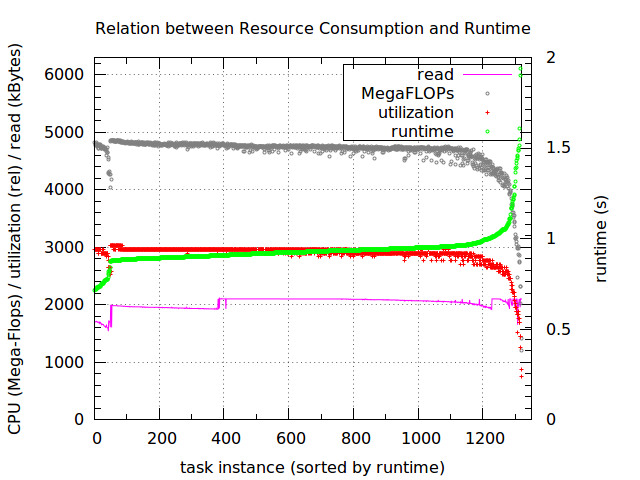
\includegraphics[width=\textwidth]{experiments/synapse_montage/rs_synapse_2mass_m101_j_6_6_mprojectpp_cpu_3}
 \end{subfigure}%
 \begin{subfigure}{.5\textwidth}
   \centering
   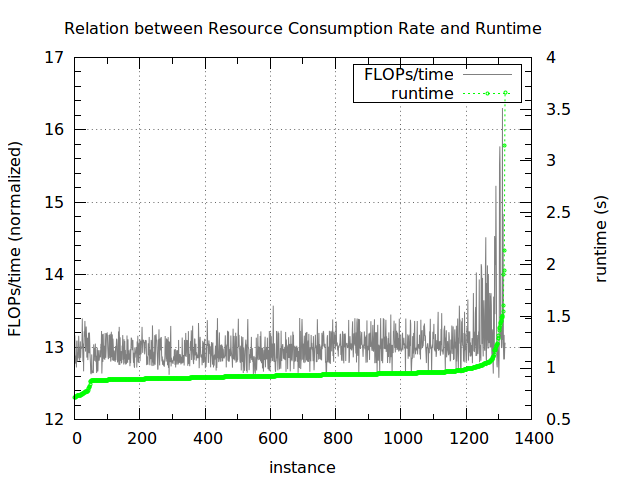
\includegraphics[width=\textwidth]{experiments/synapse_montage/rs_synapse_2mass_m101_j_6_6_mprojectpp_cpu_4}
 \end{subfigure}
  \caption {
      \footnotesize
      \B{Variation of task runtime depending on resource
      consumption:}  (left) a fraction of tasks with smaller reads consume
      less FLOPs and thus have shorter runtimes.  Overall, the CPU utilization 
      has a dominant influence on runtime, and negates the effects of lower FLOP
      consumption; (right) the resulting CPU consumption \B{rate}
      shows a strong correlation to observed application runtime,
      independent of I/O performance.
      \label{fig:synapse_cpu}
      }
 \label{fig:test}
 \end{figure}



In summary, focusing on metrics that represent resource consumption
instead of metrics that represent the \I{effects} of resource
consumption (such as runtime) allows a more accurate representation of
the application behavior on arbitrary target resources, and thus
provides adequate input to the application emulation via skeletons.
In Section~\ref{sec:Montage}, we will discuss the extent to which the
profiles provided by SYNAPSE support the results of the manual
profiling, which have been used in the skeleton emulation experiments.
% \amnote{In the later section on skeleton parameters, we need to pick
%     this up and show how that specifically confirms the manually
%     derived skeleton parameters.}


\section{Performance Evaluation}
\label{lb:Perf}
To examine and understand the differences between skeleton and real application performance, 
we select three applications (Montage, BLAST, and CyberShake PostProcessing), profile the application properties, 
produce the skeleton versions with the Application Skeleton tool, and compare the skeleton and real 
performance for each computation stage.

We chose these three applications for a variety of reasons.  First, they are applications we have familiarity with from previous research projects, either in the applications themselves or computer science problems in how to best run them on a variety of parallel and distributed systems.  Second, because fifteen stages well represent the variety of dataflow patterns that can occur in MTC applications, including gather, scatter, reduce, pipeline, and multicast~\cite{AMFS2012}. Finally, these applications and their stages are scalable and include a variety of computation/data movement ratios~\cite{ENVELOPE}.

We use 64 BG/P processors with GPFS as the shared file system. Each of the processors has a $\sim$500MB
RAM disk. Each application stage is executed with AMFORA~\cite{AMFS2013}, a parallel scripting framework on supercomputers.
With AMFORA, we can simply list all tasks of a stage in a Bash script, and instruct AMFORA to execute them (in parallel, subject to data dependencies.)

To produce skeleton applications, we first find the stage parameters,
mostly using the methods in Section~\ref{sec:manual-profiling}.
Repeated runs of the applications show very little variance in
runtime, and thus the skeleton parameters have no relevant variance
either.  The assumed normal distribution for the skeleton parameters
turned out to not always reflect reality (see for example the skewed
distribution shown in Fig.~\ref{fig:synapse_cpu} [left]), but does reflect
the correct range of measured application characteristics.
 %Another thing we learnt from the
%I/O profile is that tasks read the input files multiple times in some cases. 
% 
To compare the performance of the skeleton and real applications, we run both with AMFORA. The tasks read/write files from/to GPFS.
We run each stage five times and average the times-to-solution, though there was no significant variation in the results.

\subsection{Montage}\label{sec:Montage}

The Montage application used in this work has eight stages. We build a 6x6 degree mosaic from 1,319 2MASS image files. Each file is $\sim$2~MB. The output of the last stage, mAdd, contains
two files, each of $\sim$3.7~GB. 
%Figure~\ref{fig:Montage} shows the data flow between Montage stages, and 
Table~\ref{tb:montage-stats} shows basic statistics of each stage. 
Measured Time Avg and Measured Time Stdev show the average and the standard deviation of the time-to-solution of all tasks in each stage, respectively.

%\begin{figure}[h]
%\begin{center}
%    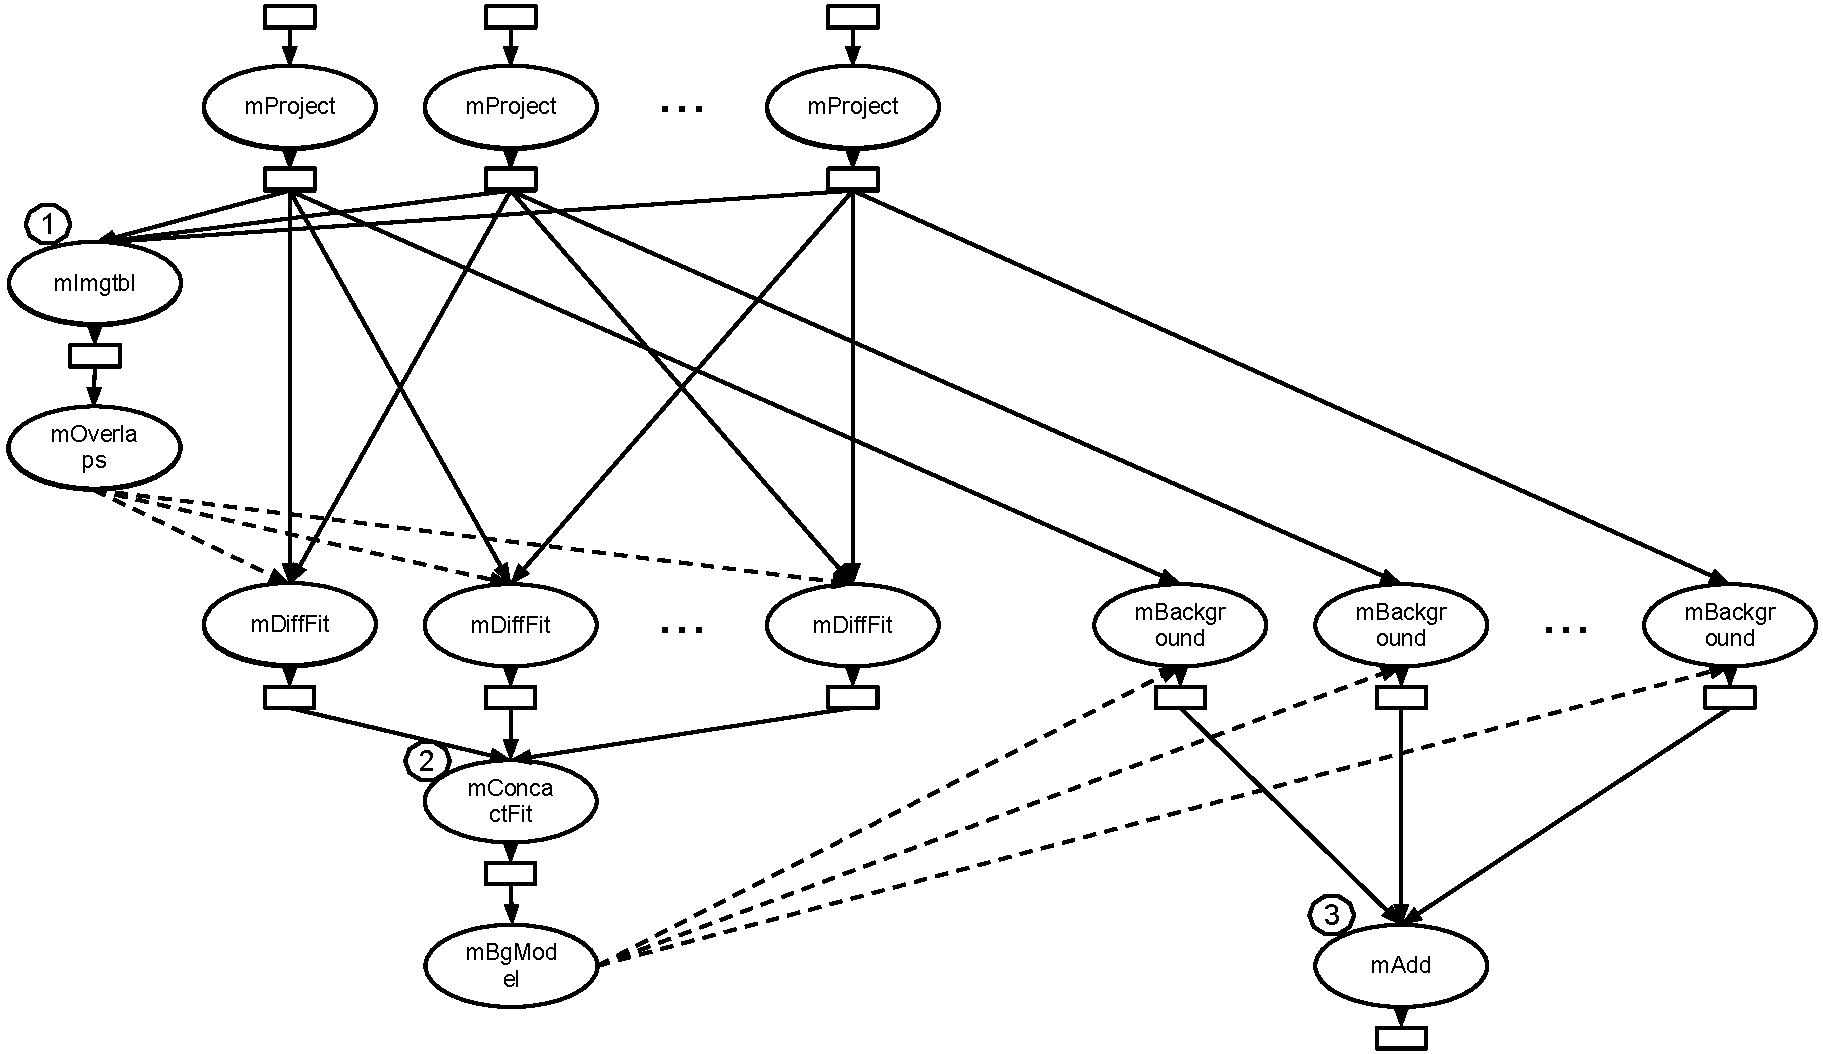
\includegraphics[width=85mm]{pictures/Montage}
%\caption {Montage dataflow. Ovals represent tasks and boxes files. Solid lines show file transfers, dashed lines show additional control flow dependencies.\zhaonote{we can remove this figure, as the flow is explained in text}
%    \label{fig:Montage}
%}
%\end{center}
%\end{figure}

\begin{table*}[ht]
\begin{center}
    \caption{Number of tasks, inputs, and outputs, and input and output size, for each Montage stage}
    \begin{scriptsize}
    \begin{tabular}{ @{} p{1.9cm} p{0.65cm} p{0.80cm} p{0.85cm} p{1.00cm} p{1.00cm} p{1.10cm} p{1.1cm} p{2.1cm}@{}}
    \toprule
    \B{Stage} & \B{\#\N Tasks} & \B{\#\N Inputs} & \B{\#\N Outputs} & \B{In\N (MB)} & \B{Out\N (MB)} & \B{Runtime Avg (s)} & \B{Runtime Stdev} & \B{Skeleton Task\N Length}\\
    \midrule
    \B{mProject   } & \HF 1319 & \HF 1319 & \HF 2594 & \HF  2800.0 & \HF 10400.0 & \HF  11.6 & \HF  2.5 & uniform \HF  11.6\\
    \B{mImgtbl    } & \HF    1 & \HF 1297 & \HF    1 & \HF  5200.0 & \HF     0.8 & \HF   N/A & \HF  0.0 & uniform \HF  30.1\\
    \B{mOverlaps  } & \HF    1 & \HF    1 & \HF    1 & \HF     0.8 & \HF     0.4 & \HF   9.1 & \HF  0.0 & uniform \HF   9.1\\
    \B{mDiffFit   } & \HF 3883 & \HF 7766 & \HF 7766 & \HF 31000.0 & \HF   487.0 & \HF   1.8 & \HF  0.6 & uniform \HF   1.8\\
    \B{mConcatFit } & \HF    1 & \HF 3883 & \HF    1 & \HF     1.1 & \HF     4.3 & \HF   2.1 & \HF  0.0 & uniform \HF   2.1\\
    \B{mBgModel   } & \HF    1 & \HF    2 & \HF    1 & \HF     4.5 & \HF     0.1 & \HF 288.0 & \HF  0.0 & uniform \HF 288.0\\
    \B{mBackground} & \HF 1297 & \HF 1297 & \HF 1297 & \HF  5200.0 & \HF  5200.0 & \HF   0.4 & \HF  0.1 & uniform \HF   0.4\\
    \B{mAdd       } & \HF    1 & \HF 1297 & \HF    2 & \HF  5200.0 & \HF  7400.0 & \HF   N/A & \HF  0.0 & uniform \HF   519\\
    \bottomrule
    \end{tabular}
    \end{scriptsize}
    \label{tb:montage-stats}
\end{center}   
\end{table*} 


%\zhaonote{explain how to set task length in each stage}
For most stages,  
we measure skeleton parameters as previously described (see Section~\ref{sec:manual-profiling}.)  However,
the input sizes for mImgtbl and mAdd exceed the maximum RAM disk size,
so we cannot use our standard technique of running the tasks with data in RAM disk. 
We observe that mAdd task's time-to-solution is proportional 
to the number of input files when that number is small (10-30), so we project the time-to-solution 
with the full input data set based on the measured time-to-solution on a smaller data set.
This method did not work well for mImgtbl in our previous study~\cite{Skeleton2013}, so for this stage, we measure the time to copy the input data set from GPFS to RAM disk by directing
the traffic to /dev/null and measure the time to copy output data from RAM disk to GPFS. 
We then subtract these two times from the time-to-solution of mImgtbl measured on GPFS and use
the result as the estimated task length. 

\begin{table*}[]
\begin{center}
    \caption{Time-To-Solution Comparison of Skeleton Montage and Real Montage (seconds)}
    \begin{scriptsize}
        \begin{tabular}{ @{} p{1.4cm}@{}p{1.10cm} p{1.00cm} p{1.3cm} p{0.80cm} p{1.2cm} p{0.9cm} p{1.1cm} p{0.75cm} p{0.9cm} @{}}
    \toprule
    & \B{mProject} & \B{mImgtbl} & \B{mOverlaps} & \B{mDiff- Fit} & \B{mConcat- Fit} & \B{mBg- Model} & \B{mBack- ground} & \B{mAdd}     & \B{Total}   \\
    \midrule
    \B{Montage } & \HF 282.3   & \HF 139.7   & \HF 10.2      & \HF 426.7      & \HF 60.1         & \HF 288.0      & \HF 107.9         &  \HF 788.8   & \HF 2103.7  \\
    \B{Stdev   } & \HF   9.7   & \HF   1.8   & \HF  0.1      & \HF   8.4      & \HF  3.4         & \HF   0.1      & \HF   2.8         &  \HF   5.9   & \HF    ---  \\
    \B{Skeleton} & \HF 281.8   & \HF 136.8   & \HF 10.0      & \HF 412.5      & \HF 59.2         & \HF 288.1      & \HF 106.2         &  \HF 781.8   & \HF 2076.4  \\
    \B{Stdev   } & \HF   7.7   & \HF   4.1   & \HF  0.1      & \HF   7.8      & \HF  2.3         & \HF   0.1      & \HF   9.9         &  \HF   6.0   & \HF    ---  \\
    \B{Error   } & \HF  -0.2\% & \HF -2.1\%  & \HF -0.2\%    & \HF  -3.3\%    & \HF -1.5\%       & \HF   0.1\%    & \HF  -1.6\%       &  \HF  -0.9\% & \HF   -1.3\%\\
    \bottomrule
    \end{tabular}
    \end{scriptsize}
    \label{tb:montage-results}
\end{center}   
\end{table*}


%%\zhaonote{explain how to set file size}
%Profiling Montage tells us that the application uses a 64-KB buffer
%size for read and write %We show one example of mBackground in Figure~\ref{fig:mBack-io}. 
%%\katznote{I don't see this in figure 3 - can you tell me where I should see 64-KB?} 
%%\zhaonote{we can see a solid red a solid blue line in the figure, they correspond to the right hand side y axis, which tells that
%%for each read/write operation, they do with a chunk size of 64 KB.}
%%The figure also indicates 
%and that the reads and writes of mBackground mostly don't overlap.
%Thus we set the interleaving option of mBackground to 0--interleave-nothing. The other Montage stages
%also have this interleaving behavior, and they are also set to 0.

%
%The input file sizes of each Montage stage are almost uniform, so we use a uniform set of  
%skeleton parameters for each stage. 
Additionally, for mDiffFit, we previously found a performance
gap between the skeleton and real mDiffFit of about 13\%~\cite{Skeleton2013} when we set the Skeleton parameters to match the
real number of files (two inputs and one output) and sizes. Examining the system call 
trace shows us that each mDiffFit task reads each input file four times instead of one. So we set 
the Skeleton parameters to eight input files, repeating the two input file names four times.
%This procedure produces good results, as shown in Table~\ref{tb:montage-results}.
%Montage tasks don't have any interleaving behavior, so the skeleton parameter for all of them is set to 0--interleave-nothing.

Using the manually-generated parameters, we measure the error of all eight stages as less than 4\%, with four under 1\%, as shown in Table~\ref{tb:montage-results}. The error for the complete application is -1.3\%.

We also compare the measured skeleton parameters as listed in
Table~\ref{tb:montage-stats} to the values derived from the system
independent profiling, as discussed in Section~\ref{ssec:si_profiling}. 
The disk I/O parameters are found in exact agreement with the manual
profiling -- the size of the input data files is fixed after all.
The SYNAPSE profiling though did automatically pick up the repeated file
reads of the mDiffFit tasks.  For the task runtimes, we calculated the
expected runtimes $t_{task}$ as follows:
 
$$
  t_{task} = f_{task} / e_{task} / u_{task} / p_{resource}^{scaled} 
$$

where $f_{task}$ is the number of FLOPs the task consumes, $e_{task}$
is the code efficiency, $u_{task}$ is the CPU utilization, and
$p_{peak}^{scaled}$ is a scalability factor which is derived from the
target CPU's peak FLOPS performance, scaled by the actually observed
performance in performance benchmarks.  The latter value, for the
specific BG/P used for the experiments, is set to 
$\frac{191 GFlops/sec}{557 GFlops/sec} = 0.34$,
based on a 2008 HPC challenge entry for that
target
machine\footnote{\url{http://www.hpcchallenge.org/custom/index.html?lid=103&slid=229}}.
The code efficiency and CPU utilization are measured on an
architecturally very different x86 CPU.

\begin{table*}[h]
\begin{center}
    \caption{runtime observation vs. runtime prediction}
    \begin{scriptsize}
        \begin{tabular}{@{}l@{}rrr@{}}
    \toprule
    \B{Stage}       & \B{measurement} & \B{prediction} &  \B{deviation} \\
    \midrule
    \B{mProject   } &        11.6 &       8.54 &       1.35 \\
    \B{mImgtbl    } &         N/A &      27.41 &        N/A \\
    \B{mOverlaps  } &         9.1 &       7.36 &       1.23 \\
    \B{mDiffFit   } &         1.8 &        N/A &        N/A \\
    \B{mConcatFit } &         2.1 &        N/A &        N/A \\
    \B{mBgModel   } &       288.0 &     386.69 &       0.74 \\
    \B{mBackground} &         0.4 &       0.62 &       0.64 \\
    \B{mAdd       } &         N/A &    1477.54 &        N/A \\
    \bottomrule
    \end{tabular}
    \end{scriptsize}
    \label{tb:prof-compare}
\end{center}   
\end{table*}


\tablename~\ref{tb:prof-compare} shows that
while most runtimes predicted by system
independent profiling have the correct order of magnitude,
they deviate from the values observed via manual profiling by
about 25\%, either positively or negatively.  
This is not surprising, given the effort that is
usually spent on optimizing the core computational libraries and
application codes toward a specific target architecture, which makes
the code efficiency and CPU utilization not easily portable from one
architecture and operating system to another.  The manual
profiling on any target architecture thus gives, naturally, more
precise runtime values for that architecture, but the automated
profiling via system independent variables provides reasonable
estimates for resources consumptions on resources for which manual
profiling is difficult or impossible to perform. 
% \katznote{need to follow-up on this in conclusions section.}

%\begin{figure}[h]
%\begin{center}
%    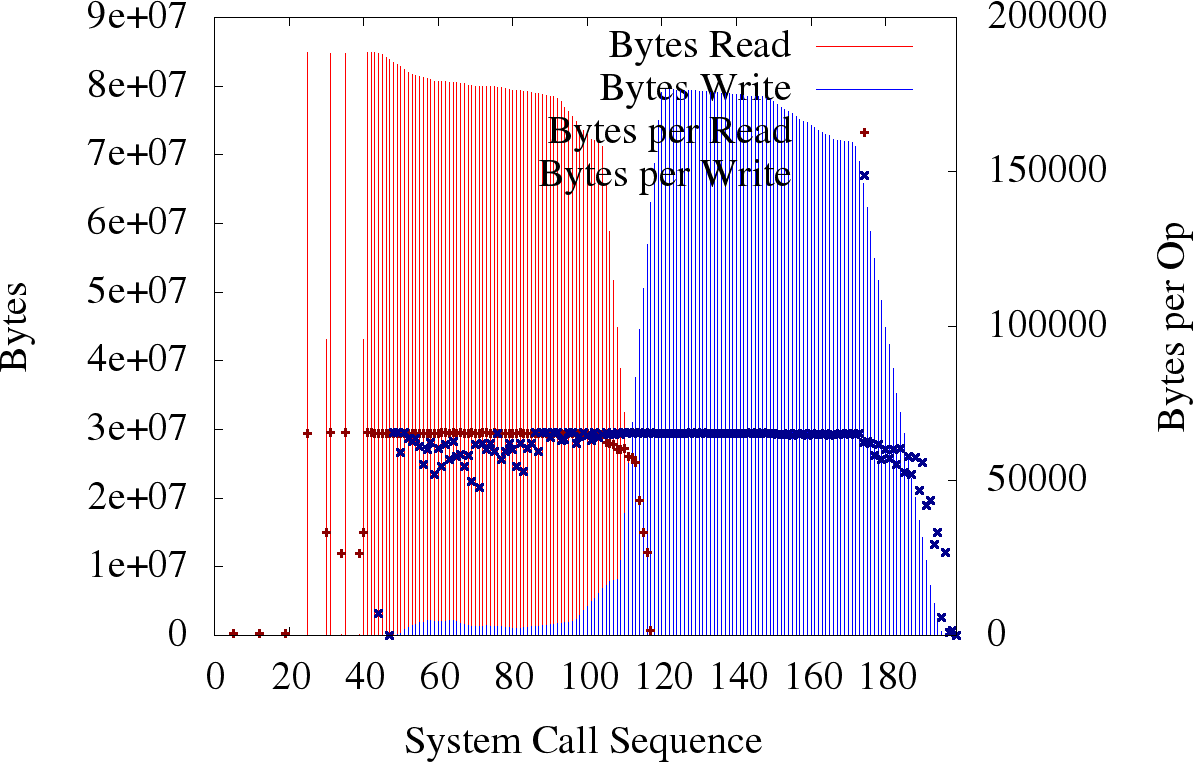
\includegraphics[width=85mm]{pictures/mBack-io}
%\caption {I/O related system calls of all mBack tasks aligned with the sequence order. The left axis shows 
%the accumulated I/O amount at a given system call. The right axis shows the I/O traffic amount per system
%call.\zhaonote{we can delete this figure to save space}
%    \label{fig:mBack-io}
%}
%\end{center}
%\end{figure}


\subsection{BLAST}

BLAST is a widely used sequence alignment tool. The version we use here is parallelBLAST~\cite{ParallelBlast}, which has four stages. The first stage partitions a 3.8 GB data base into slices. The second stage formats each 
partition. The third-stage tasks query each formatted database partition with an identical set of query sequences. The
fourth stage merges the partial results from all partitions into an output file for each query sequence file 
(since there could be multiple query sequences in one file). %In our experiments, we use the latter three stages of BLAST for profiling and comparison. 
%\zhaonote{oops, I forgot to measure the partition stage, we didn't take partition into
%account in Envelope or AMFS work as it can not run in parallel. We can measure it on other computers now. Shall we
%do that?} \katznote{yes please}
%
%
In our experiments, we run the first 1,024 queries of the NRxNR test case. 
%Figure~\ref{fig:BLAST} shows the data flow and task dependencies between BLAST stages. 
Table~\ref{tb:blast-stats}
shows the basic statistics of each BLAST stage. 

\begin{table*}[t]
\begin{center}
    \caption{Number of tasks, inputs, and outputs, and input and output size, for each BLAST stage}
    \begin{scriptsize}
    \begin{tabular}{ @{} p{1.4cm} @{}p{0.65cm} p{0.80cm} p{0.95cm} p{0.85cm} p{1.00cm} p{1.10cm} p{1.1cm} p{2.8cm}@{}}
    \toprule
    \B{Stage} & \B{\#\N Tasks} & \B{\#\N Inputs} & \B{\#\N Outputs} & \B{In\N (MB)} & \B{Out\N (MB)} & \B{Runtime Avg (s)} & \B{Runtime Stdev} & \B{Skeleton Task\N Length}\\
    \midrule
    \B{split   } & \HF    1 & \HF    1 & \HF   64 & \HF  3800 & \HF 3800 & \HF   0.0 & \HF  N/A &         \HF             0 \\
    \B{formatdb} & \HF   64 & \HF   64 & \HF  192 & \HF  3800 & \HF 4400 & \HF  41.9 & \HF  0.1 & uniform \HF            42 \\
    \B{blastp  } & \HF 1024 & \HF 4096 & \HF 1024 & \HF 70402 & \HF  966 & \HF 109.2 & \HF 14.9 & normal  \HF [109.2, 14.9] \\
    \B{merge   } & \HF   16 & \HF 1024 & \HF   16 & \HF   966 & \HF  867 & \HF   4.4 & \HF  4.1 & normal  \HF    [4.4, 4.1] \\
    \bottomrule
    \end{tabular}
    \end{scriptsize}
    \label{tb:blast-stats}
\end{center}   
\end{table*}

%\begin{figure}[h]
%\begin{center}
%    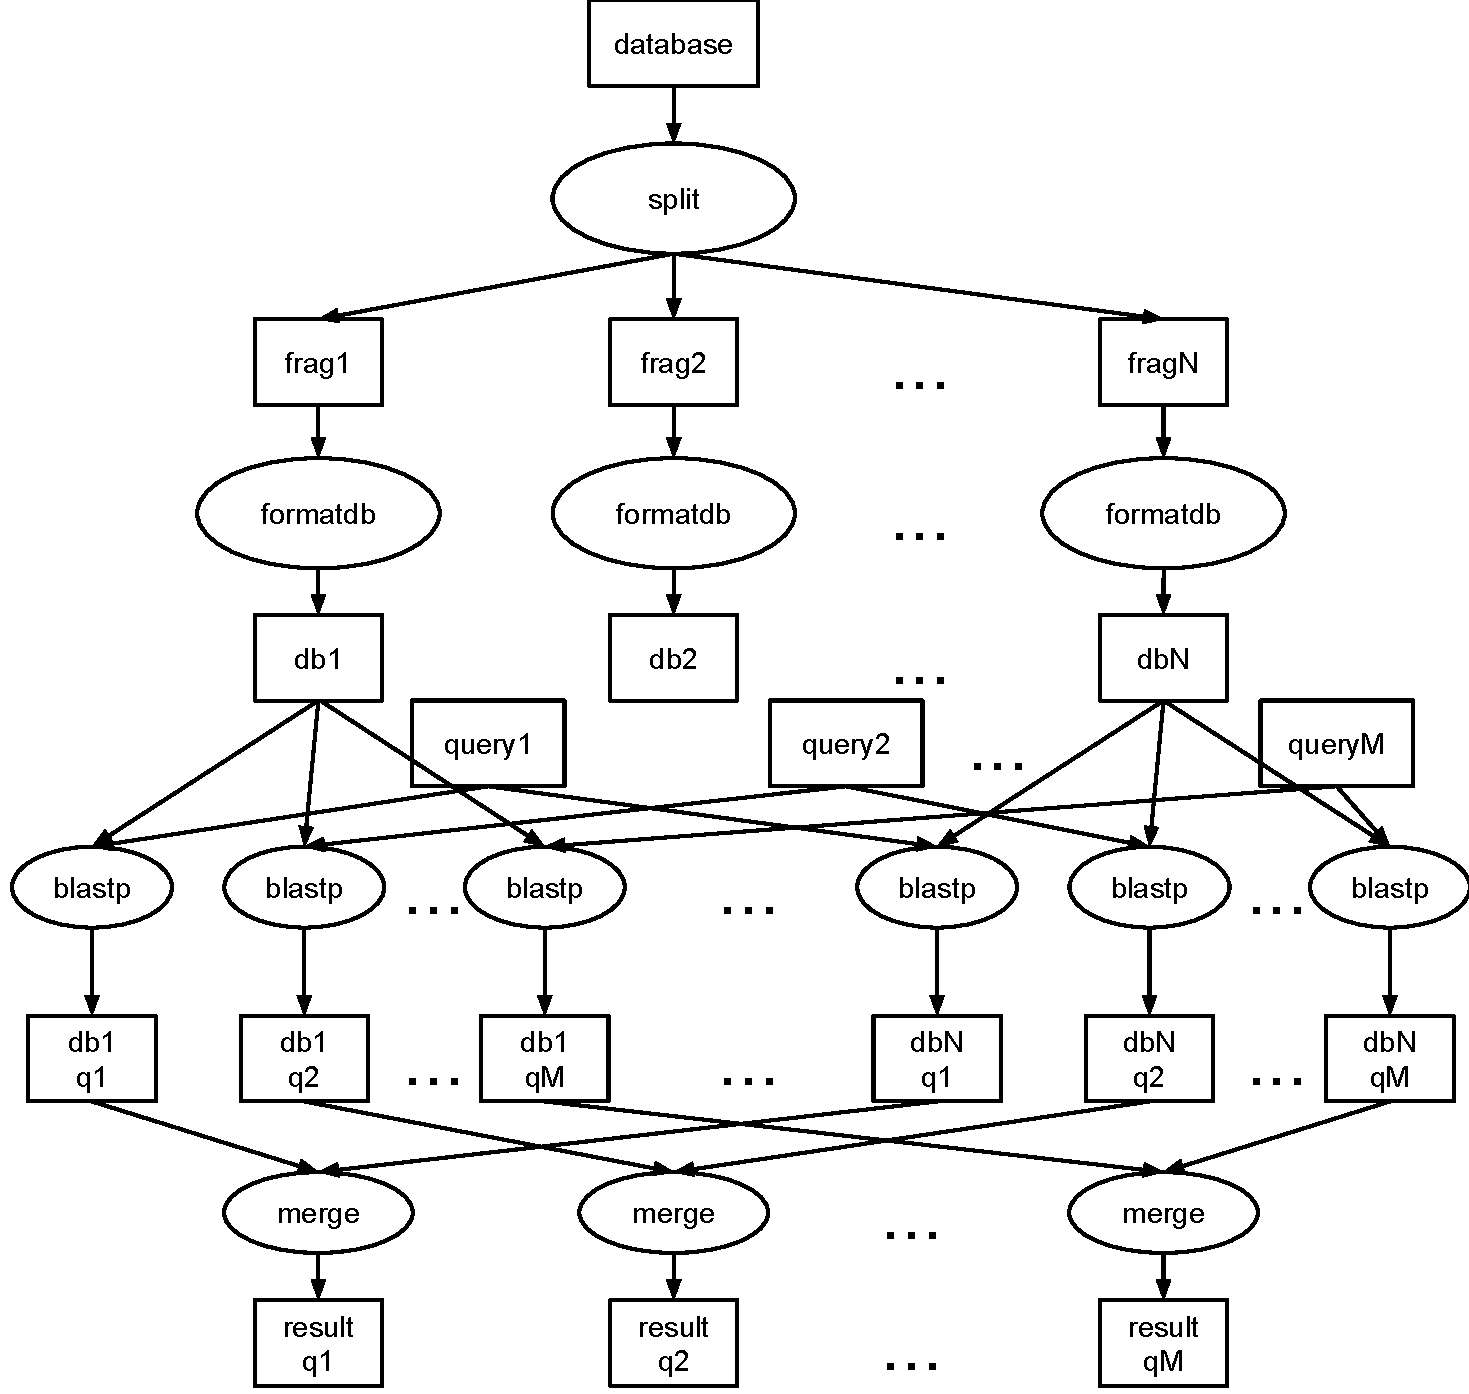
\includegraphics[width=85mm]{pictures/BLAST}
%\caption {BLAST dataflow. Ovals represent tasks and boxes files. Solid lines show file transfers.\zhaonote{we can remove this figure, as the flow is explained in text}
%    \label{fig:BLAST}
%}
%\end{center}
%\end{figure}

In general, we measure the task parameters as described in Section~\ref{sec:manual-profiling}.
The split stage has a single task does no significant 
computation, so we simply set the split task's length to zero. 


Also, all tasks of the four stages of BLAST read each input file just once. Each formatdb task reads one input file of $\sim$60~MB 
and writes three output files of size 56~MB, 16~MB, and 1~MB, respectively. We simplify the skeleton formatdb task with three
output files with identical size of 21~MB, since this results in the same amount of metadata operations and I/O traffic.

%\zhaonote{explain how to set buffer size and interleaving option}
%The split task uses 4096 Bytes as its read and write buffer size. 
%Profiling of the formatdb stage showed us that each formatdb task reads the database with a 64-KB buffer. However,
%there are roughly 500,000 writes with a size of hundreds of Bytes.
%%, as shown in Figure~\ref{fig:formatdb-io}. 
%With our
%previous Skeleton implementation, we could not specify a buffer size and had to run the real and skeleton applications
%with all data in RAM to get close to real performance. With the new implementation, we are able to set the formatdb read buffer to 64~KB and the write buffer 
%to 512~Bytes. 
Finally, 64 concurrent formatdb tasks each with $\sim$500,000 small writes can run for hours on
GPFS. So when we compare the Skeleton and real formatdb, we run the both with data caching in RAM disk. For blastp and merge stage, we run the tasks with data in GPFS.

%\begin{figure}[h]
%\begin{center}
%    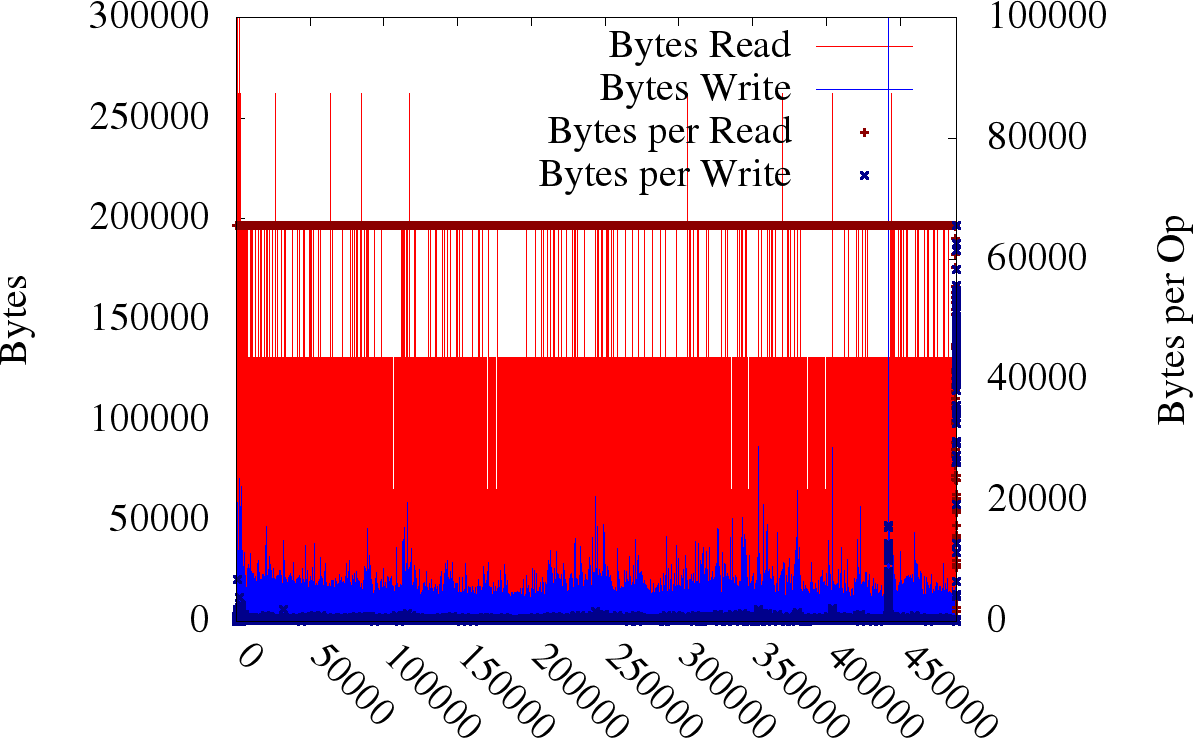
\includegraphics[width=85mm]{pictures/formatdb-io}
%\caption {I/O related system calls of all formatdb tasks aligned with the sequence order. The left axis shows 
%the accumulated I/O amount at a given system call. The right axis shows the I/O traffic amount per system
%call.
%    \label{fig:formatdb-io}\zhaonote{we can delete this figure to save space}
%}
%\end{center}
%\end{figure}

%For all tasks in the four stages of BLAST, we see an interleaved computation and I/O pattern. 
%%In formatdb, % as shown in Figure~\ref{fig:formatdb-io},
%%each task reads a sequence, formats that sequence, and writes the result to output files. 
%%Thus, there are $\sim$500,000 writes with a size of hundreds of Bytes.
%%In blastp, the task reads a sequence, computes the similarity score between this sequence and every sequence in one database partition, and writes the result. 
%%The merge task also interleaves its work. 
%So we set the interleaving options as 3--interleave-all. 
%%The skeleton tasks read
%%a piece of the input file, sleep for some time, and write a piece of the output, repeating these steps until all work is done.

\begin{table}[t]
\begin{center}
    \caption{Time-To-Solution Comparison of Skeleton BLAST and Real BLAST (seconds)}
    \begin{scriptsize}
        \begin{tabular}{ @{} p{1.4cm} p{1.2cm} p{1.4cm} p{1.4cm} p{1.4cm} p{1.4cm} @{} }
    \toprule
             & \HF \B{split}  & \HF \B{formatdb} & \HF \B{blastp} & \HF \B{merge} & \HF \B{Total}\\ 
    \midrule
    \B{BLAST   } & \HF 74.4   & \HF 82.1     & \HF 1996.3 & \HF 35.9  & \HF 2188.7 \\
    \B{Stdev   } & \HF  0.6   & \HF  1.7     & \HF    6.0 & \HF  1.1  & \HF    --- \\
    \B{Skeleton} & \HF 72.9   & \HF 81.6     & \HF 2028.9 & \HF 36.3  & \HF 2219.7 \\
    \B{Stdev   } & \HF  2.7   & \HF  0.3     & \HF    1.2 & \HF  0.5  & \HF    --- \\
    \B{Error   } & \HF -1.9\% & \HF -0.6\%   & \HF 1.6\%  & \HF 1.1\% & \HF  1.4\% \\
    \bottomrule
    \end{tabular}
    \end{scriptsize}
    \label{tb:blast-results}
\end{center}   
\end{table}

\begin{table*}[t]
\begin{center}
    \caption{Number of tasks, inputs, and outputs, and input and output size, for each CyberShake Postprocessing stage}
    \begin{scriptsize}
        \begin{tabular}{ @{} p{1.5cm} @{} p{0.80cm} p{0.80cm} p{0.80cm} p{1.00cm} p{1.00cm} p{1.2cm} p{1.1cm} p{2.5cm}@{}}
    \toprule
    \B{Stage} & \B{\#\N Tasks} & \B{\#\N Inputs} & \B{\#\N Outputs} & \B{In\N (MB)} & \B{Out\N (MB)} & \B{Runtime Avg (s)} & \B{Runtime Stdev} & \B{Skeleton Task\N Length}\\
    \midrule
    \B{Extract} & \HF  128 & \HF  130 & \HF  256 & \HF  5400 & \HF 11000.0 & \HF  6.4 & \HF  2.2 & uniform \HF         6.39\\
    \B{Seis   } & \HF 4096 & \HF 4352 & \HF 4096 & \HF 11000 & \HF    96.0 & \HF 26.9 & \HF 13.3 & normal  \HF [26.9, 13.3]\\
    \B{PeakGM } & \HF 4096 & \HF 4096 & \HF 4096 & \HF    96 & \HF     1.4 & \HF  0.2 & \HF  0.1 & uniform \HF         0.23\\
    \bottomrule
    \end{tabular}
    \end{scriptsize}
    \label{tb:cybershake-stats}
\end{center}   
\end{table*}


%\zhaonote{results}
Table~\ref{tb:blast-results} compares the measured performance of the Skeleton BLAST and real BLAST.
The error of each stage is -1.9\%, -0.6\%, 1.6\%, and 1.1\%, respectively. 
%The measurements of the skeleton blastp stage uses the
%normal task length distribution. (Our attempt with a uniform distribution had a larger error: -2.7\%.) 
The overall application error is 1.4\%.

\subsection{CyberShake}


CyberShake~\cite{SCEC07, SCEC10} finds the probabilistic peak ground movement at a physical site caused by a set of potential earthquakes. The first step of the application generates strain Green tensors (SGTs), by running two MPI calculations that each produce one SGT file for the physical site. The second step is Postprocessing, which performs a parameter sweep over two dimensions: ruptures that could affect the site, and the variations of every rupture. For each rupture, Postprocessing extracts a subset of the SGT files, and then for each variation of that rupture, Postprocessing calculates a computational seismogram and finds the peak ground motion in the seismogram.
In our experiments, we run the first 128 Extract tasks, and 4,096 Seis and PeakGM tasks.
%Figure~\ref{fig:cybershake} shows the data flow and task dependencies of CyberShake Postprocessing. 
Table~\ref{tb:cybershake-stats} shows the basic statistics of each CyberShake Postprocessing stage. 

\begin{table}[t]
\begin{center}
    \caption{Time-To-Solution Comparison of Skeleton CyberShake and Real CyberShake (seconds)}
    \begin{scriptsize}
        \begin{tabular}{ @{} p{1.5cm} p{1cm} p{1cm} p{1.2cm} p{1cm} @{} }
    \toprule
                   & \B{Extract} & \B{Seis}   & \B{PeakGM} & \B{Total}  \\ 
    \midrule
    \B{CyberShake} & 571.5       & 2386.5     & 81.5       & 3039.4     \\
    \B{Stdev     } &  15.9       &   40.8     &  1.5       &    ---     \\
    \B{Skeleton  } & 586.3       & 2443.3     & 83.3       & 3112.9     \\
    \B{Stdev     } &   1.5       &    4.9     &  2.7       &    ---     \\
    \B{Error     } & 2.6\%       & 2.4\%      & 2.3\%      & 2.4\%      \\
    \bottomrule
    \end{tabular}
    \end{scriptsize}
    \label{tb:cybershake-results}
\end{center}   
\end{table}


%\begin{figure}[h]
%\begin{center}
%    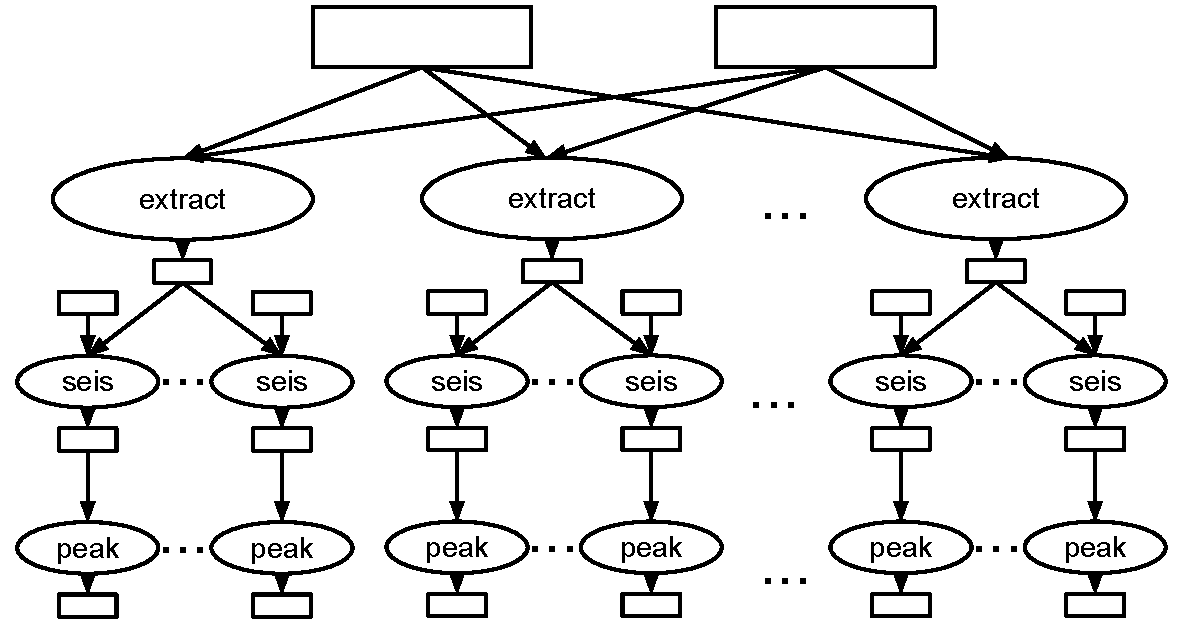
\includegraphics[width=85mm]{pictures/SCEC-PostProcessing}
%\caption {CyberShake Postprocessing Dataflow Pattern \zhaonote{we can remove this figure, as the flow is explained in text}
%    \label{fig:cybershake}
%}
%\end{center}
%\end{figure}


%\zhaonote{explain how to set task length}
%We wanted to run the tasks in every stage with data cached RAM and use the time-to-solution as task length in Application Skeletons. 
We generally use the previously discussed methods to determine skeleton parameters.
However, each Extract task needs to access the two SGT files and a rupture variation file, and the SGT file's size is 5.4 GB, which is too large for a compute node's RAM disk.
So instead we ran the first 50 tasks manually on each compute node in sequence order, measured the times-to-solution and 
then computed the average and standard deviation. 
Although the tasks access data on GPFS, running one task at a time excludes the overhead  incurred  by highly concurrent I/O operations. 
%The Seis and PeakGM tasks' I/O fits in RAM disk, so we directly measure the time-to-solution of each task. For task lengths of the Seis
%stage, we use a normal distribution specified by the average and standard deviation. The task lengths of the PeakGM tasks is uniform.

%\zhaonote{explain how to set file size}
In addition, the two SGT input files for each Extract task are about 2.7 GB each. %When we specify the skeleton Extract task's input size as 2.7 GB, the operating
%system failed 
%\katznote{what does this mean?  Is this a BGP limitation?  Or an AMFORA limitation? Is it really the OS?} 
%\zhaonote{It is the ZeptoOS on BGP. It can not access the file size that is larger than 1,000,000,000 bytes, though it can read the file content. I am not exactly sure if it is the ZeptoOS or the BGP system.}
%when the task accesses file metadata since 2.7 GB is beyond the file size that the OS supports. Also, 
We observe from the strace profile that
an Extract task does not read the whole input file; rather it reads only  about 200 MB. So we %decided to 
set the skeleton parameters for two SGT input
files with  size of 200~MB, which %. This %removes the too large file issue and it 
preserves the I/O traffic that actually happens
in an Extract task. 
%We set the output files of the Extract, Seis, and PeakGM stage to a size of 34~MB, 36~KB, and 240~Bytes, respectively.
%The interleaving option for all three stages is set to 0--interleave nothing.

%\zhaonote{one skeleton limitation of file mapping}
In the real CyberShake Postprocessing application, the file usage of the Extract output files (a subset of the SGT files) in the Seis stage is not uniform. Some files are used more than  others. Computer scientists who want to implement an automatic file usage-based runtime 
replication system might find it infeasible to specify such unbalanced file usage with the current Application Skeletons implementation. One
solution for this problem is the external file option, which can customize file mappings to tasks and  can generate
uneven file usage.
However, we simply set the Seis tasks to read each pair of Extract output files evenly, which suffices to give performance matching that of the real application on our test system.
%In our Skeleton settings for the Seis stage, we simplify this problem by unifying the input file usage. 
%\katznote{what does this sentence mean?}
%\zhaonote{In our experiment settings,  the 4096 Seis task consumes each output pair of Extract (128 in total) 32 times. While ideally, one can use the external mapper to specify the exact file usage as the real Seis stage.}
%\katznote{see if my edit above is ok.  If so, please remove these comments}

Table~\ref{tb:cybershake-results} presents the comparison between the skeleton CyberShake Postprocessing applications and the real applications. 
All three stages have errors under 3\%, with a total error of 2.4\%.


\section{Using Application Skeletons}\label{lb:using}
%\zhaonote{this section is new, please review}
Here, we show examples of using application skeletons (with manually generated parameters) to study four system improvements: data caching, task scheduling, I/O tuning, and resilience. 
Various system optimizations were implemented with the AMFORA~\cite{AMFS2013} system. 
The experiments were carried out on the Google Compute Engine (GCE) environment. 
Throughout all these experiments, we used ``n1-highmem-2'' instances, which have two vCPU cores and 13~GB RAM. 


\subsection{Data Caching}
Data caching is a common technique when application data fits in RAM. Here, we run real-mProjectPP from Montage and skeleton-mProjectPP.
with files located on PVFS and AMFORA to show improved performance. PVFS and AMFORA use four GCE compute nodes.
The real-mProjectPP workload finishes in 285.2~s with PVFS and 100.9~s on AMFORA.
Skeleton-mProjectPP runs in 273.7~s on PVFS and 101.3~s on AMFORA.
The data-caching optimization on skeleton-mProjectPP workload (63.0\%) has identical improvement on the real-mProjectPP workload (64.6\%). This example shows that skeleton applications can be used for designing, implementing, and testing the system optimizations, in place of the more complex real applications.


\subsection{Task Scheduling}
In this example, we seek to show the time-to-solution improvement of data-aware scheduling over the FIFO (first-in, first-out) scheduling algorithm.
We implement both scheduling algorithms in the AMFORA task engine and run both  real-mProjectPP  and skeleton-mProjectPP
on 16 compute nodes of GCE. The real-mProjectPP workload and skeleton-mProjectPP workload both have insignificant improvements of 0.7\% and 1.6\%, respectively, because of the nature of the mProjectPP tasks. 
The ratio of I/O to task length is the root cause of these insignificant improvements.
When we modify the skeleton-mProjectPP with a 5x larger input file size, we can see a 16.4\% time-to-solution improvement with data-aware scheduling over FIFO.  This shows an additional benefit of skeleton applications: we can use them in place of real applications and easily modify them to better understand when system optimizations will have a significant effect.

\subsection{I/O Tuning}
For applications that have highly concurrent and frequent metadata operations, using multiple metadata servers can improve the overall application performance~\cite{GIGA+, PVFS2009}.
We built AMFORA with a configurable metadata server design, and we want to use the mProjectPP workload to verify that multiple metadata servers can actually improve
the performance with a single metadata server.
With 16 compute nodes of GCE,  real-mProjectPP and skeleton-mProjectPP show only  1.1\% and 1.2\% improvements, respectively,  with multiple metadata servers over a single metadata server, although
the improvement is stable. 
The marginal improvement is again due to the nature of the mProjectPP tasks: the task execution is dominated by computation, which makes  improvement in metadata access negligible.
When we modify the skeleton-mProjectPP task with a 10x shorter task length, we see a 31.2\% improvement with multiple metadata servers over a single metadata server.  Similar to the last example, this shows a benefit of using skeleton applications over real applications.

\subsection{Resilience Mechanism}
In the AMFORA system resilience design, we proposed a dynamic replication approach that combines both task re-execution and file replication. 
The decision is made by calculating the expected recovery time using each replication strategy and choosing the one with lower overhead.
Originally, we used the mBackground stage from Montage since it has a mix of tasks: some tasks' output files should be recovered by re-execution, while
some should be recovered by file replication. 
We want to show that this dynamic replication approach has the best recovery performance over either pure re-execution or pure file replication when there
is a node failure during execution.
We ran the workload on various scales on GCE, but the improvements are marginal. 
The reason is that the recovery overhead difference of mBackground tasks is not significant, so even if we make the right decision for every task, the accumulated
improvement is still not significant.
To prove the benefit of this dynamic resilience strategy, we need to show  a more significant improvement of the recovery performance. We first profiled the mBackground tasks' time-to-solution and I/O parameters, and generated a skeleton-mBackground workload with similar performance as real-mBackground. We then provisionally executed the skeleton-mBackground workload with AMFORA and recorded which files were replicated by re-execution and replications.
We next modified the skeleton-mBackground workload to have 10x longer tasks for the tasks whose output files
should be replicated, and 10x larger output files for the tasks whose output files should be recovered by re-execution. 
In other words, we magnified the penalty of the wrong replication decision.
With this modified skeleton-mBackground work load, we see an increased improvement of 9.1\%, 4.4\%, and 4.9\% on 4, 16, and 64 compute nodes of GCE, respectively.


%\section{Related Work}\label{lb:RFwork}
%
%We believe that the idea of using application skeletons, particularly for overall system performance, is relatively novel.  In generally, we accept that researchers have been using application replacements for experiments for a long time, and some of those replacements were certainly tunable in one way or the other. The distinction in our work is that the Skeletons provide that capability in a systematic way, being tunable to a range of diverse application, including multi-stage applications, with the promise to preserve the significant part of the application's behavior. This is why we do not list much related work here: the problem space is pervasive, but attempts to solve it systematically are rare, particularly for distributed applications. 
%
%Examples of benchmarking/analysis work in a parallel (not distributed) context include the Berkeley Dwarfs~\cite{dwarfs} (also called `motifs') and the related OpenDwarfs~\cite{6868650}.  Such work has at its core the idea that there is a key computational or data movement kernel that is responsible for most of the application's performance, and that that kernel can be extracted and used to represent the full application, at least in terms of performance.
%
%An alternative method is from Sodhi et al.~\cite{Sodhi:2008:PPS:1355774.1355777}, who developed a tool called performance skeletons.   
%These are short running parallel MPI programs with performance meant to fractionally represent the performance of the full applications.  Unlike the dwarf work, this assumes that the work done by applications is spread through out the application (not in a single kernel).
%This idea of fractional versions of parallel applications is also unlike our work, which produces simplified and scalable versions of full distributed applications. 
%Sodhi's work does overlap ours in its approach to automatically capturing the execution behavior of an application and automatically generating a synthetic skeleton program that reflects that execution behavior, but is also fairly different, as it focuses on single system MPI applications that do not have disk I/O.  
%
%Skel~\cite{Skel} uses a similar idea to understand the I/O performance of parallel applications on supercomputers. Users can extract 
%the I/O behavior from an application, then produce a skeletal application that mimics the I/O operations and pattern by specifying
%a Skel configuration file. The produced skeletal application can run on ADIOS~\cite{ADIOS}. 
%
%The work that is probably closest to ours is WGL~\cite{WGL}, which abstracts an application from a dataflow point of view and lets users generate a Swift script for a potentially distributed workflow application by 
%describing the dataflow patterns between stages.  Since there is some institutional overlap between
%the WGL developers and Skeleton developers and because both overlap the Swift team, it's likely that informal discussions carried some of this concept from WGL to Skeletons, though there is a nine-year gap between the projects.
%
%An example of loosely related work is by Holl et al.~\cite{Holl:2013:SSS:2534248.2534251}, who have studied how to store and share parameters values for shared workflows, an idea that could be applied to skeleton values.
%
%
%%Algorithmic motifs (skeletons)~\cite{foster1990parallel} abstracts parallel application with an algorithmic approach, and let users build parallel
%%programs based on the algorithmic skeletons.

\section{Conclusion and Future Work}\label{lb:Con}

Application Skeletons are motivated by the difficulties of real application access and modification that computer scientists who work on tools and systems have. We use a top-down approach to abstract a distributed application in Application Skeletons: applications 
are composed of a number of stages, while each stage is composed of a number of tasks, with task parameters specified at the stage level. The stage is built on a versatile task design that can handle different task types, various buffer
sizes, multiple input/output files, and different interleaving scenarios. Overall, one can create easy-to-access, easy-to-build, easy-to-change, and easy-to-run bag-of-tasks, 
(iterative) map-reduce, and (iterative) multistage workflow applications. Our Application Skeleton  tool is designed to work with mainstream workflow
frameworks and systems: Bash Shell, Pegasus, and Swift.

%\katznote{Also, we might say that now once a skeleton code represents a real code, it can be easily distributed (through just the parameters) to make middleware and tool experiments repeatable/reproducible, and it can make it easy to scale experiments - some of this also perhaps should go in the intro or abstract as motivation}
Representing an application by a set of skeleton parameters means that the skeleton application  can be easily repeated and easily shared, making 
middleware and tool experiments more reproducible.  This leads in two directions: computer science education and computer science research.

In computer science education, skeleton applications can be used by students to allow them to understand important properties of parallel and distributed applications.  Simple skeletons can be used as instantiations of application abstractions, and more complex skeletons can be used in place of real applications.

In computer science research, including but not limited to the educational process,
skeleton application and changes to their parameters can be used to
study particular aspects of system performance.
Computer scientists can then focus on the system or tools they are building.
%, and in some cases, the optimizations of skeleton applications can
%also be applied to the real applications. 
%\zhaonote{Not very confident with the last sentence, as the skeleton application's I/O trace is not exactly the same as the real ones'. Need to think about this.} 
%\katznote{and as I said, we should think about making some of these points in the abstract and introduction, too|}
%\zhaonote{yes, fixed for now, please review}

We have shown that the skeleton applications generated by our Application Skeleton tool have performance close to that of the real applications.  We profiled three representative distributed applications---Montage, BLAST, CyberShake PostProcessing---to understand their computation and I/O behavior and then derived parameters required to specify
the skeletons.  

We also investigated the tradeoffs between manually-measured, system dependent
skeleton parameters and automated, system independent skeleton
parameters. Manual, system dependent parameters are more precise than system
independent metrics, but are also harder to obtain.  The system independent
parameters, however, represent reasonable estimates for resource consumption on
systems where manual profiling is difficult or impossible to perform.

%\katznote{we may need to say something somewhere about why we keep saying distributed but actually use a single parallel systems.  If so, we would need to say this here, in the abstract maybe, and in the introduction - perhaps something like that these applications can and are run on both distributed and parallel systems, and our skeletons can similarly be run on both, but that we use parallel systems for testing because they are simpler, but our results should carry over to distributed systems.  Do you think this is true?  In any case, we should think about where we say distributed...} 
%\zhaonote{yes I agree, I think one of the reasons we measure it on parallel system is the performance stability. For example, it is hard for OSG to have identical performance between two experiments with exactly the same settings.  put a few words here, please review.}

%\zhaonote{we can remove the next two paragraphs. The first one is arguing that we use parallel systems, but now we are running on GCE also. The next explains some tech details}
%Our measurements are on a parallel system rather than a distributed
%environment such as OSG or XSEDE, since a homogeneous supercomputer delivers better performance stability, 
%while a distributed environment's properties can vary dramatically, potentially
%leading to significant unpredictable noise in the measurements. However, our work has been motivated by both parallel and distributed systems, and we believe that our tools are directly useful on distributed systems as well as the parallel systems we have used so far.


%%\katznote{maybe say that our previous work showed this to be generally true, but not always, and here, we discovered some issues we had missed previously.} 
%%\zhaonote{add the following paragraph to address the above comment, please review.}
%Our previous work showed this profiling approach generally, worked with a few exceptions. 
%We looked at those exceptions and found some cases we did not address very well, including task length distribution (BLAST-blastp), 
%interleaved computation and I/O (BLAST-formatdb), and overlooked repeated reads over the same input files (Montage-mDiffFit). We have now improved our methods, and we show that we can now determine skeleton parameters that more accurately describe applications.

The Application Skeleton tool can produce skeleton applications that correctly capture important distributed properties of real applications but 
are much simpler to define and use.
Comparing performance (with manually-measured skeleton parameters) shows overall errors of  -1.3\%, 1.5\%, and 2.4\%  for Montage, BLAST, and CyberShake PostProcessing, respectively.
At the stage level, fourteen out of fifteen stages have errors of less than 3\%,
ten have errors less than 2\%, and four have errors of less than 1\%.  The
standard deviations for all experiments is consistently well below 10\%, (mostly
below 5\%), and is also consistent between application and skeleton measurements.

The four examples of system improvements (data caching, task scheduling, I/O tuning, and resilience mechanism) 
showed that using skeleton applications simplifies the process of system optimization design, implementation, and verification, and that by making small changes to the skeletons, we can highlight the effects of optimizations.

%In the near future, we will release the Application Skeleton code as open source, and invite users and contributors from a wider community to try it and expand it.
%Later, we plan the following: 
%\katznote{changes here?}
%\zhaonote{add ``cloud environments'' in the last item.}
The Application Skeleton code is available as open source at \url{https://github.com/applicationskeleton/Skeleton}~\cite{skeleton-software-v1.2} under the MIT license. We invite the community to try it and to contribute to it.

We plan the following in the near future:
\begin{itemize}
\item {} Use application trace data to produce skeleton applications, ideally purely from the trace data but initially from a combination of trace data and user guidance.
\item {} Investigate how well Skeletons represent applications when
    configured with system independent parameters, as derived by SYNAPSE.
\item {} Determine a way to represent the computational work in a task that when combined with a particular platform can give an accurate runtime for that task.
\item {} Support concurrent tasks that need to run at the same time to exchange information.
\item {} Test on distributed systems where latencies, particular file usage, and other issues may be more important than on the parallel systems and cloud environments.
\item {} Allow more varieties of I/O behavior for parallel tasks than just process 0 performing all I/O.
%\katznote{add an item about testing on distributed systems where latencies and particular file usage and other issues may be more important than on the parallel systems we have used so far}
%\zhaonote{add one item, please review.}
%\item{} Work within the AIMES project to integrate Application Skeletons with the AIMES framework. \katznote{not sure this is really meaningful to readers - let's see what the AIMES folks say}
%\katznote{I'm not sure what the rest of this means} 
%\zhaonote{tryied to explain why we need to integrate, nevermind, we can remove it.}
%to extend AIMES's application coverage by providing applications with a wide range of characteristics.
%\zhaonote{Mention integration with AIMES framework. do we have an AIMES reference? Does the above sentence look ok?}
\end{itemize}

\section*{Acknowledgments}

This work is part of the AIMES project, supported by the U.S. Department of Energy 
under the ASCR awards DE-FG02-12ER26115,
DE-SC0008617, and DE-SC0008651.
It has benefited from discussions with Matteo Turilli, Jon Weissman, Michael Wilde, Lavanya Ramakrishnan, and Simon Caton.
Computing resources were provided by the
Argonne Leadership Computing Facility and Google. Work by Katz was supported by 
the National Science Foundation while working at the Foundation.  Any 
opinion, finding, and conclusions or recommendations expressed in this
 material are those of the author(s) and do not necessarily reflect 
 the views of the National Science Foundation.
 

%% \section{}
%% \label{}

%% If you have bibdatabase file and want bibtex to generate the
%% bibitems, please use
%%
\bibliographystyle{elsarticle-num} 
\bibliography{Skeleton}

%% else use the following coding to input the bibitems directly in the
%% TeX file.

%% \begin{thebibliography}{00}

%% \bibitem{label}
%% Text of bibliographic item

%% \bibitem{}

%% \end{thebibliography}
\end{document}
\endinput
%%
%% End of file `elsarticle-template-num.tex'.
